\documentclass[a4paper]{report}
\usepackage[T1]{fontenc}
\usepackage[utf8]{inputenc}
\usepackage[francais]{babel}   
\usepackage[top=2cm, bottom=2cm, left=2cm, right=2cm]{geometry}
\usepackage{graphicx}
\usepackage{url}
\usepackage{soul}
\usepackage{setspace}
\usepackage{listings}
\usepackage{multirow}
\usepackage[colorlinks=true,bookmarksopen     = true]{hyperref}
\usepackage{ccaption} 

\hypersetup{
linkcolor= black
}

\lstset{
language=Java,
basicstyle=\footnotesize,
numbers=left,
numberstyle=\normalsize,
numbersep=7pt,
}


\title{	\fbox{
	\begin{minipage}{\textwidth}
		\begin{Large}
			\begin{center}
				Spécification et Modélisation
			\end{center}  
		\end{Large}
	\end{minipage}	
	}
	\begin{minipage}{\textwidth}
    \center
    
\includegraphics[width=15cm]{img/divers/logo}
	\end{minipage}
	}
\author{Alexandre \bsc{Hamann}, Clément \bsc{Herledan}, Yannick \bsc{Guern}, Clément \bsc{Perreau}}
\date{S6P 2013}

\setcounter{tocdepth}{5}
\setcounter{secnumdepth}{5}		
 
\begin{document}

\maketitle

\makeatletter
\renewcommand*\l@chapter[2]{%
  \ifnum \c@tocdepth >\m@ne
    \addpenalty{-\@highpenalty}%
    \vskip 1.0em \@plus\p@
    \setlength\@tempdima{1.5em}%
    \begingroup
      \parindent \z@ \rightskip \@pnumwidth
      \parfillskip -\@pnumwidth
      \leavevmode \bfseries
      \advance\leftskip\@tempdima
      \hskip -\leftskip
      #1\nobreak\ 
       \leaders\hbox{$\m@th
        \mkern \@dotsep mu\hbox{.}\mkern \@dotsep
        mu$}\hfil\nobreak\hb@xt@\@pnumwidth{\hss #2}\par
      \penalty\@highpenalty
    \endgroup
  \fi}
\makeatother

\makeatletter
\renewcommand\l@section[2]{%
  \ifnum \c@tocdepth >\z@
    \addpenalty\@secpenalty
    \addvspace{1.0em \@plus\p@}%
    \setlength\@tempdima{-2em}%
    \begingroup
      \parindent \z@ \rightskip \@pnumwidth
      \parfillskip -\@pnumwidth
      \leavevmode {\bfseries
      \advance\leftskip\@tempdima
      \hskip -\leftskip
      #1}\nobreak\ 
      \leaders\hbox{$\m@th\mkern \@dotsep mu\hbox{.}\mkern \@dotsep mu$}
     \hfil \nobreak\hb@xt@\@pnumwidth{\hss #2}\par
    \endgroup
  \fi}
\makeatother

\tableofcontents

~
\newpage

\part{Spécification}

\chapter*{Introduction}
\addcontentsline{toc}{chapter}{Introduction}

\begin{onehalfspace}
	Dwarves Manager est un jeu de gestion qui prend place dans un univers fantastique classique. Le joueur est aux commandes d'une mine dans laquelle des nains (créatures fantastiques de la mythologie scandinave) travaillent à extraire toute sorte de ressources. Le but du jeu est de gérer cette petite entreprise, et de l'aider à remplir ses objectifs.

	Le joueur doit pour cela recruter des nains, mettre en place des structures pour répondre à leurs besoins, afin de maximiser la productivité. Il définit également les zones que les nains doivent excaver pour récolter des ressources. 
Le but du jeu, dans un premier prototype sera d'acquérir une certaine quantité de ressources, avant la fin d'un temps imparti.
\end{onehalfspace}

\begin{figure}[bh!]
    \center
    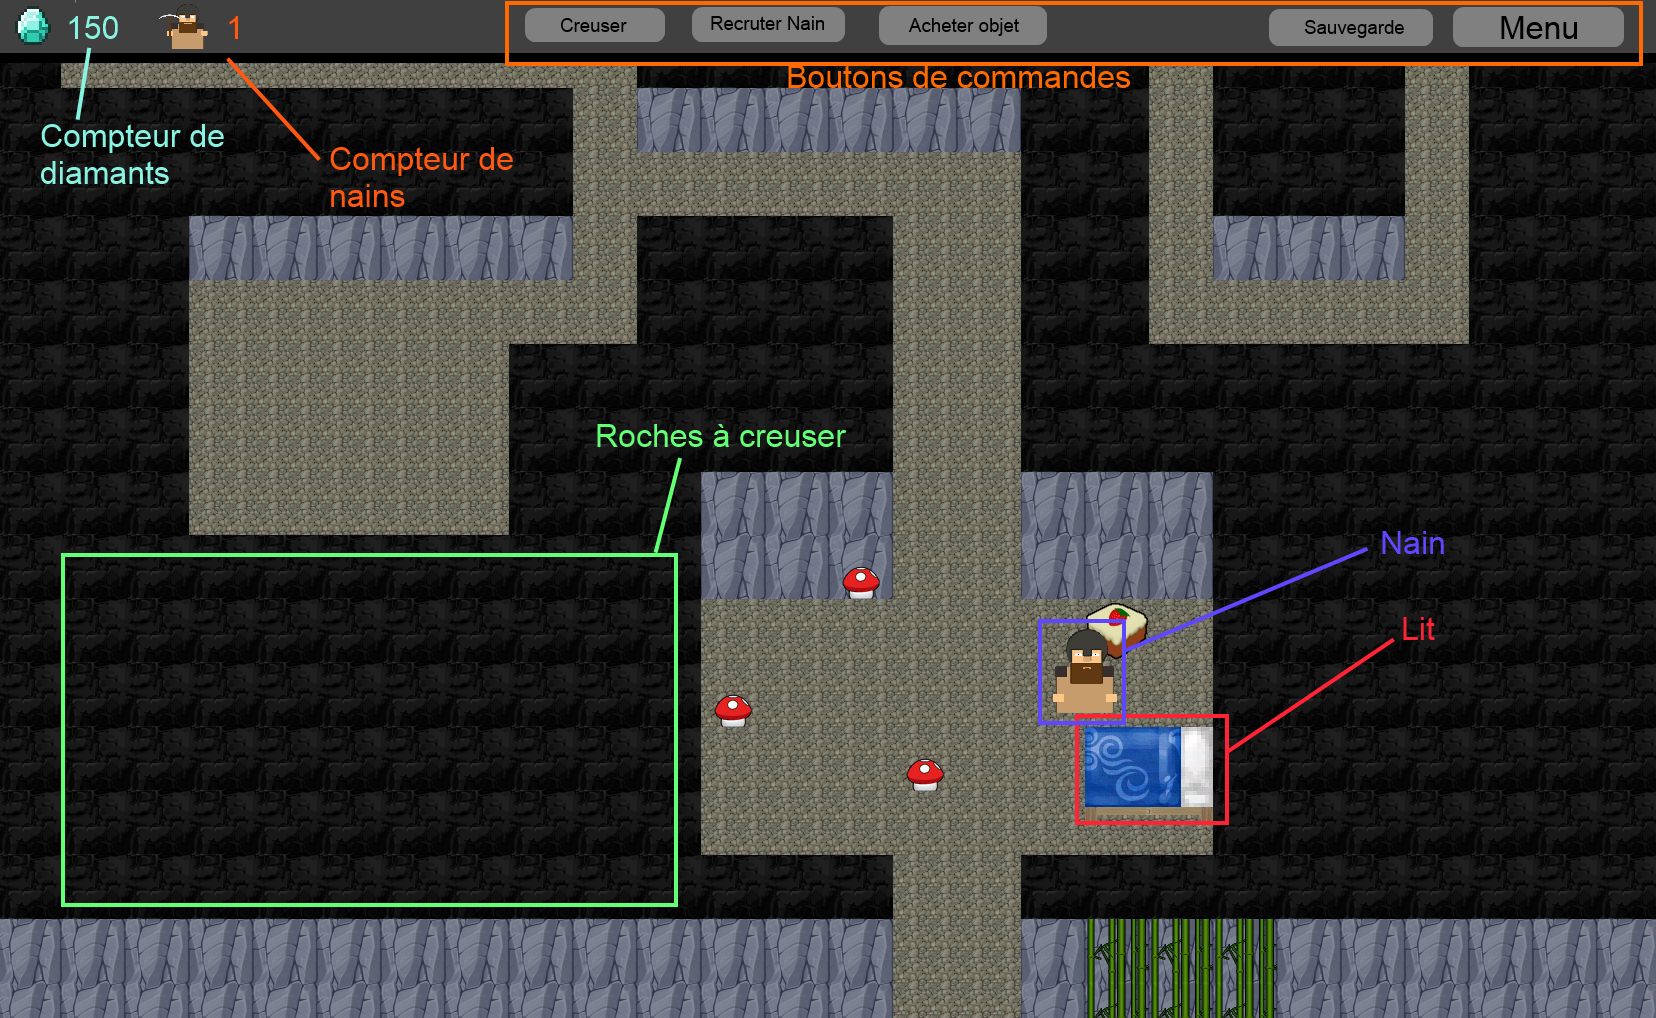
\includegraphics[width=15cm]{img/divers/visu}
    \caption{Aspect prévu du jeu}
\end{figure}
~
\newpage

\chapter*{UseCase}
\addcontentsline{toc}{chapter}{UseCase}

\begin{center}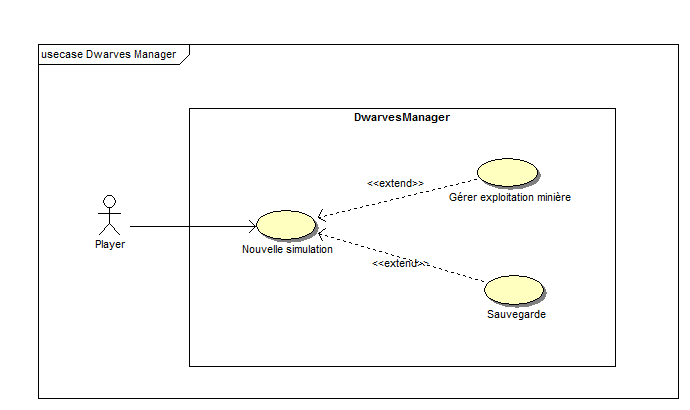
\includegraphics[scale=0.5]{img/spec/usecase}\end{center}

\section*{Nouvelle simulation :}
Le joueur sélectionne un scénario ou une partie enregistrée, afin de lancer une 	nouvelle instance de simulation.

\section*{Gérer exploitation minière :}
Le joueur gère l'exploitation.
Cela inclue la possibilité de recruter/renvoyer de nouveaux nains, placer des 	objets pour leur confort. 
Le joueur défini également les zones du monde à creuser.

\section*{Sauvegarde :}
Sauvegarde de l'état de la simulation dans un fichier.

\newpage
\chapter*{Scénario}
\addcontentsline{toc}{chapter}{Scénario}


\section*{Nouvelle Simulation}

\begin{tabular}{|c|c|p{9cm}|}
\hline
& \multicolumn{2}{c|} {\textbf{Nouvelle Simulation}}  \\ \multirow{2}{*}{\textbf{Sommaire d'identification}} & 
\multicolumn{2}{p{10cm}|} {\raggedright Le joueur sélectionne un scénario ou une partie enregistrée, afin de lancer une 
nouvelle instance de simulation.}\\
\hline 
		& \multirow{2}{*}{Nominal}   & * Le joueur choisit une scénario\\ && * Le joueur valide son choix\\ \cline{2-3}
\multirow{3}{*} {\textbf{Description scénarios}}		& \multirow{2}{*}{Alternatif} & * Le joueur choisit une partie sauvegardée \\ && * Le joueur valide son choix\\ \cline{2-3}
		& \multirow{2}{*}{Erreur}     & * Le joueur choisit une partie sauvegardée \\ && * Le niveau ne peut pas être chargé(niveau inexistant)\\\cline{2-3}
		
\hline
\end{tabular}


\begin{figure}[htp]%
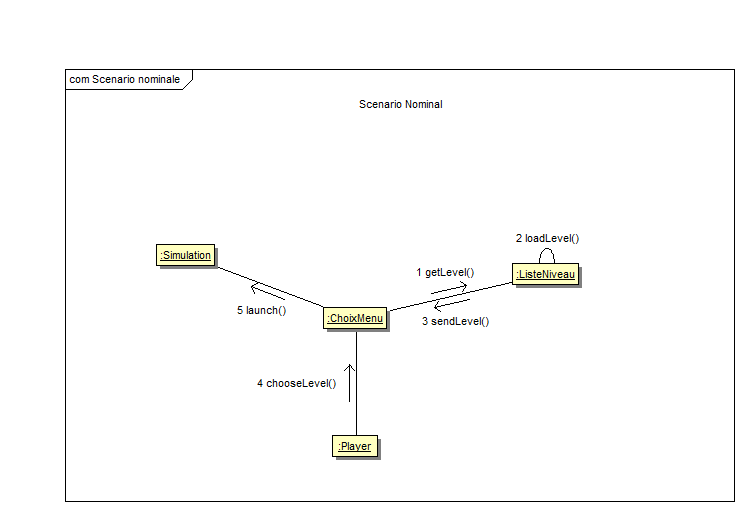
\includegraphics[width=\columnwidth]{img/spec/nominal}%
\caption{Scénario nominal}%
\label{}%
\end{figure}


\begin{figure}[htp]%
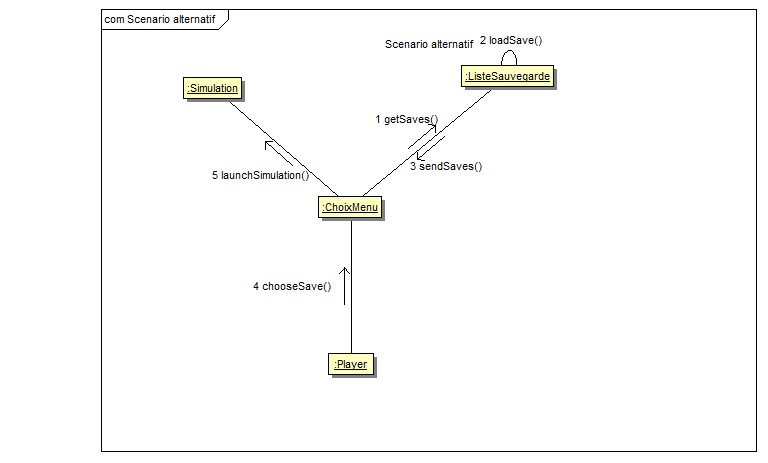
\includegraphics[width=\columnwidth]{img/spec/alternatif}%
\caption{Scénario alternatif}%
\label{}%
\end{figure}

\begin{figure}[htp]%
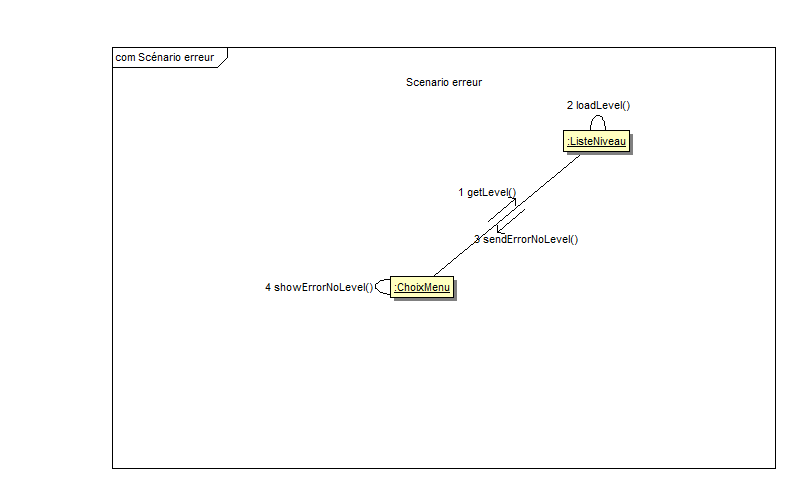
\includegraphics[width=\columnwidth]{img/spec/erreur}%
\caption{Scénario erreur}%
\label{}%
\end{figure}

\section*{Gérer exploitation minière}


\begin{tabular}{|c|c|p{9cm}|}
\hline
& \multicolumn{2}{c|} {\textbf{Nouvelle Simulation}}  \\ \multirow{3}{*}{\textbf{Sommaire d'identification}} &
\multicolumn{2}{p{10cm}|} {\raggedright * Le joueur gère l'exploitation.}\\&
\multicolumn{2}{p{10cm}|} {\raggedright * Cela inclut la possibilité de recruter/renvoyer de nouveaux nains, placer des		objets pour leur confort. }\\&
\multicolumn{2}{p{10cm}|} {\raggedright * Le joueur définit également les zones du monde à creuser.}\\ 
\hline
\multirow{13}{*}{\textbf{Sommaire d'identification}}
		& \multirow{8}{*}{Nominale} 
				&* Le joueur recrute un nain\\ &
				&* Le joueur place un lit\\  &
				&* Le joueur définit une zone à miner \\ &
				&* Le nain commence à miner \\ &
				&* Le nain fatigué, rejoint son lit pour dormir \\ &
				&* Le nain repart travailler et fini de miner \\ &
				&* Le nain récolte des diamants pour le joueur \\ &
				&* Le joueur ayant récolté assez de diamants remporte la partie \\
				\cline{2-3}
		& \multirow{6}{*}{Alternatif} 
				&* Le joueur recrute un nain\\ &
				&* Le joueur définit une zone à miner \\ &
				&* Le nain commence à miner \\ &
				&* Le nain fatigué refuse de continuer à travailler (pas de lit pour dormir) \\ &
				&* Le joueur perd la partie parce que le temps qui lui était alloué est écoulé \\ 
				\cline{2-3}
				\hline
\end{tabular}


\begin{figure}[htp]%
\includegraphics[width=\columnwidth]{img/spec/sd_nominal}%
\caption{Scénario nominal}%
\label{}%
\end{figure}

\begin{figure}[htp]%
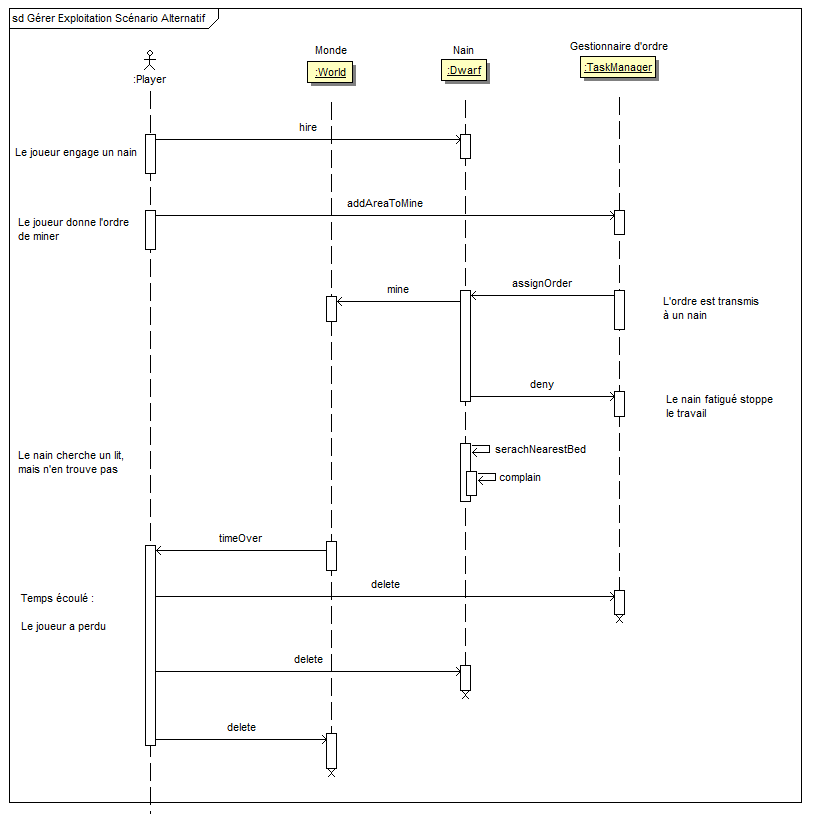
\includegraphics[width=\columnwidth]{img/spec/sd_alternatif}%
\caption{Scénario alternatif}%
\label{}%
\end{figure}


\newpage

\section*{Sauvegarde}



\begin{tabular}{|c|c|p{9cm}|}
\hline
\multirow{2}{*}{\textbf{Sommaire d'identification}} & \multicolumn{2}{c|} {\textbf{Sauvegarde }}  \\ &
\multicolumn{2}{p{10cm}|} {\raggedright Sauvegarde de l'état de la simulation dans un fichier.}\\
\hline
\multirow{6}{*} {\textbf{Description scénarios}} 
		& \multirow{3}{*} {Nominale}   & * Le joueur rentre un nom \\ && * Le joueur valide\\ && * Sauvegarde effectuée \\ \cline{2-3}
		& \multirow{4}{*} {Erreur}     & * Le joueur rentre un nom \\ && * Le joueur valide\\ && * Échec de la sauvegarde (Nom invalide, ou chemin inaccessible en écriture) \\ \cline{2-3}
		
\hline
\end{tabular}

\begin{figure}[htp]%
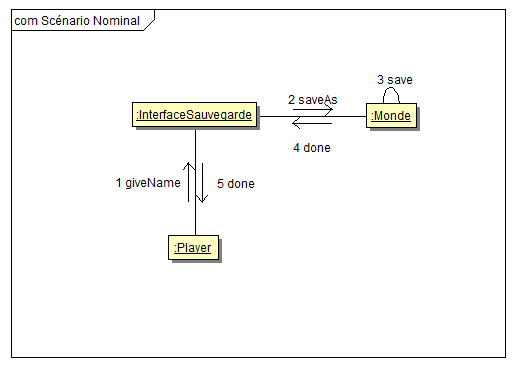
\includegraphics[width=\columnwidth]{img/spec/sauvegardeNominal}%
\caption{Scénario nominal}%
\label{}%
\end{figure}

\begin{figure}[htp]%
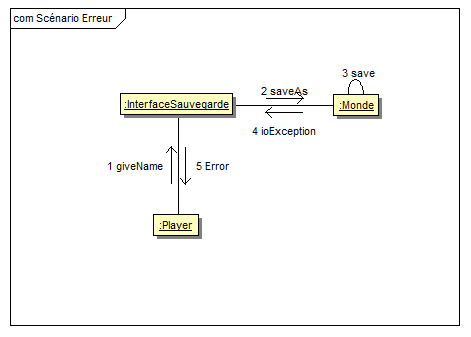
\includegraphics[width=\columnwidth]{img/spec/sauvegardeErreur}%
\caption{Scénario erreur}%
\label{}%
\end{figure}

\newpage
\part{GameDesign}
\vspace{0.2cm}

\chapter*{Introduction}
\addcontentsline{toc}{chapter}{Introduction}

Le but de cette partie est de décrire précisément les mécaniques de jeu que nous souhaitons implémenter, de décrire le style artistique et graphique du jeu, ainsi que son contexte imaginaire.

\vspace{0.2cm}
\chapter*{Mécaniques de jeu}
\addcontentsline{toc}{chapter}{Mécanique de jeu}

\vspace{0.2cm}
\bsc{Personnages :}
\vspace{0.2cm}

\begin{description}
\item[Le nain mineur :]Le nain mineur travaille à extraire les ressources dans les zones décrites par le joueur. Il a besoin de se reposer régulièrement et de se détendre à la taverne, et aussi d'une pioche en bon état pour miner.
\item[Le nain artisan :]Le nain artisan répare et fabrique des pioches pour les mineurs.
\item[Le nain tavernier :]Le nain tavernier sert les bières à la taverne
\end{description}

\vspace{0.2cm}
\bsc{Pièces et Objets :}
\vspace{0.2cm}

\begin{description}
\item[Le dortoir :]Le dortoir est la pièce de la mine où sont installés les lits où dormiront les nains.
\item[La taverne :] La taverne est l'endroit où viennent se détendre les nains après une dure journée de labeur.  La taverne a besoin d'un comptoir, d'un fût à bière et d'au moins une table pour fonctionner.
\item[L'atelier :] L'atelier est l'antre du nain artisan. Il y a une enclume et un râtelier pour permettre au nain artisan de travailler. Avant d'aller travailler, les nains viennent y chercher leur pioche, et au retour du travail ils viennent y déposer leur pioche dans un râtelier prévu à cet effet.
\end{description}

\vspace{0.2cm}
\bsc{Les besoins :}
\vspace{0.2cm}

\begin{description}
\item[Le sommeil :]Pour répondre à un manque de sommeil, le nain doit dormir dans un lit dans un dortoir.
\item[La bière :] Les nains doivent aller à la taverne boire des bières régulièrement.
\end{description}

Chaque nain recruté est différent et possède une certaine prédisposition à la fainéantise et à l'alcoolisme déterminée aléatoirement par une loi normale. Un nain peut donc être paresseux et passer tout son temps à dormir, ou encore passer tout son temps à boire des bières à la taverne, mais cela restera relativement rare.

\vspace{0.2cm}
\bsc{Gestion du personnel :}
\vspace{0.2cm}

Le joueur est libre de renvoyer n'importe lequel des nains, néanmoins, il devra payer une prime de licenciement. De même quand on embauche un nain, il faudra payer une prime d'embauche. 

Remplacer un nain fainéant par exemple peut se révéler très coûteux, surtout si son remplaçant n'est pas meilleur.

Régulièrement, il faut aussi payer les salaires, recruter trop de nains peut vite mener une exploitation à la faillite, et lorsque le minerai s’épuise, il faut envisager de lourd plans sociaux.

\chapter*{Contrôles :}
\addcontentsline{toc}{chapter}{Contrôles}

Les actions du joueur sont relativement limitées. Il lui est possible de recruter de nouveaux nains, de délimiter les zones à miner, de délimiter des pièces, de placer des objets de mobilier et de confort.

Toute la subtilité du jeu relève du fait que tous les contrôles sont indirects, le joueur n'a pas à sélectionner et à donner un ordre précis à chacun des personnages, il définit juste les zones de travail et aménage l'espace de ses employés.


\newpage
\chapter*{Direction artistique :}
\addcontentsline{toc}{chapter}{Direction artistique}

Nous avons réalisé quelques dessins des personnages dans un style minimaliste dès le début de projet afin de pouvoir imaginer au plus tôt l'aspect final du jeu. Voir figure ~\ref{Personnages}, page~\pageref{Personnages}.

Néanmoins, la réalisation de toutes les ressources graphiques n'étant pas notre priorité, les personnages seront les seuls éléments que nous dessineront. Nous tenterons bien sur de réunir des ressources graphiques et sonores qui collent au mieux à l'univers du jeu.

\begin{figure}
    \center
    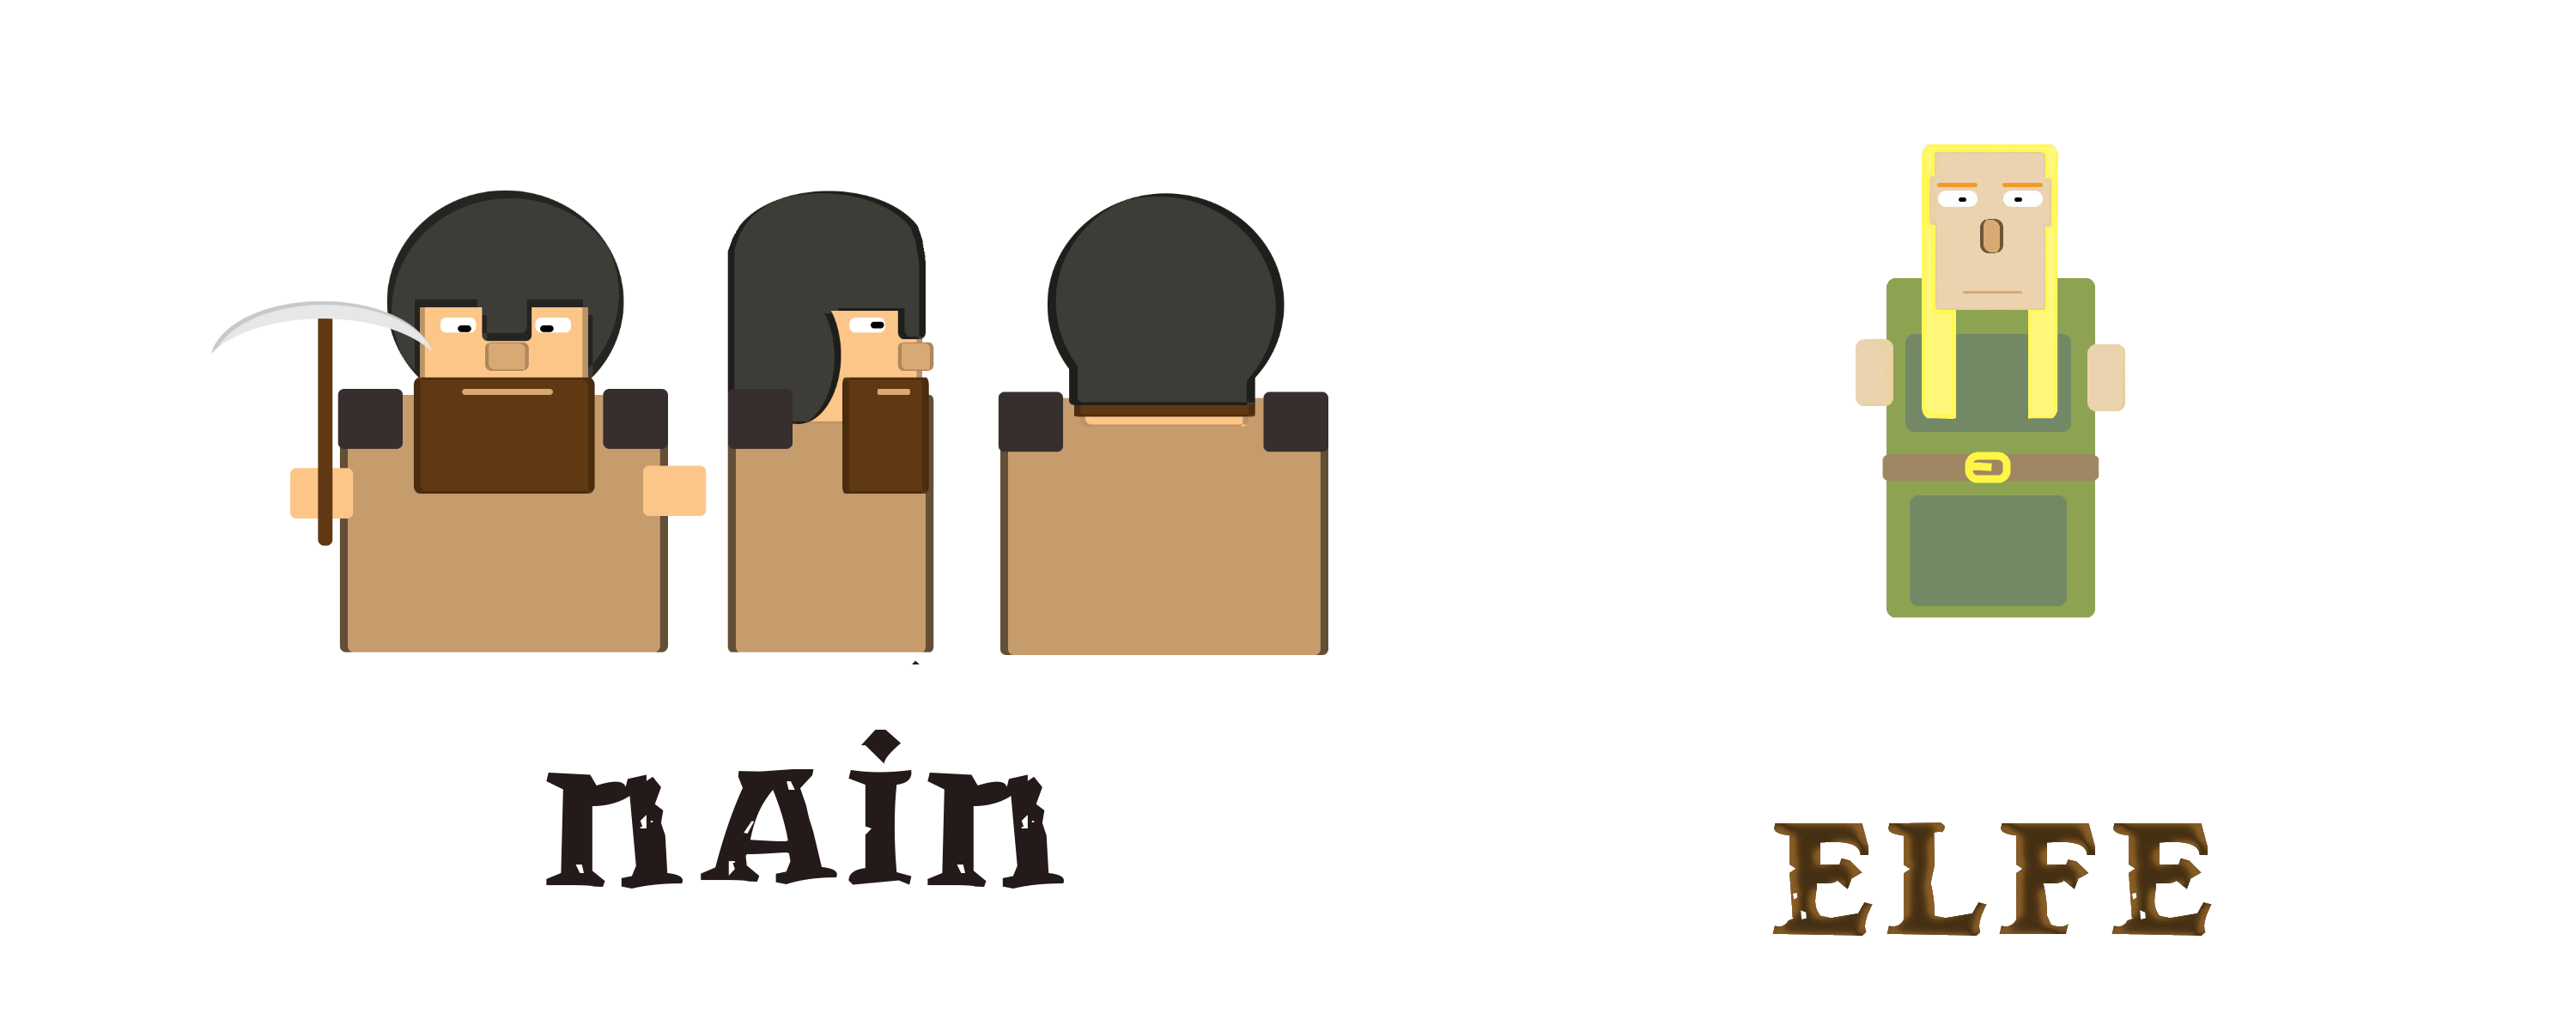
\includegraphics[width=15cm]{img/divers/chara}
    \caption{Style des personnages}
		\label{Personnages}
\end{figure}

\newpage

\chapter*{Background :}
\addcontentsline{toc}{chapter}{Background}

\section*{Les nains :}

Le nain est une créature humanoïde imaginaire souterraine de petite taille, dont la figure actuelle est principalement issue de la mythologie nordique et des croyances germaniques médiévales.


Mythologie nordique : 

Les nains (dvergr en vieux norrois) sont des créatures vivant sous terre, dans les pierres ou les montagnes, ils sont originellement des vers trouvés dans la dépouille du géant Ymir, auxquels les dieux donnent forme humaine et 
intelligence, mais qui du fait de leur origine continuent à vivre sous terre et dans les pierres. Les nains sont souvent rusés, et se caractérisent par leur habileté, surtout en tant que forgerons. En effet, ils sont responsables
de la création de la majorité des attributs divins, dont le marteau de Thor. Les textes mythologiques ne donnent aucune information relative à la taille des nains, et il n'y a pas de raison de penser qu'ils étaient de petite taille.
Cette représentation apparaît dans les sagas tardives, où ils sont décrits petits et généralement laids. La croyance en des nains caricaturaux, de petite taille et généralement malins et mystérieux, est restée dans le folklore 
populaire germanique après la christianisation.


Cet aspect des nains est repris dans une grande majorité d'histoire fantastique et de jeux. L'un des exemples est le seigneur des anneaux où les nains sont des créatures humanoïdes de petite taille, vraisemblablement entre
1 mètre 20 et 1 mètre 50. Ils sont robustes, font d'excellents combattants et sont dotés d'une grande résistance à la faim et à la douleur. Leur espérance de vie moyenne est de deux cent cinquante ans. Un aspect important de
leur physique est leur barbe, qu'ils ne rasent jamais et qui est portée par les hommes comme par les femmes. Les Nains minent et travaillent les métaux précieux et la pierre avec un talent inégalé dans la terre du milieu.
Ils sont également de grands forgerons, créateurs de nombreuses armes de légende. Ils sont aussi réputés pour l'usage de hache comme arme de prédilection.


\begin{figure}[hb!]
    \center
    \includegraphics[scale=2]{img/divers/gimli}
    \caption{Une représentation de nain : Gimli de la Communauté de l'Anneau}
		\label{Nain}
\end{figure}

\clearpage

\newpage
\part{Spécification technique}

\chapter*{Choix technologiques}
\addcontentsline{toc}{chapter}{Choix technologiques}

Nous avons choisi de développer Dwarves Manager en Java avec le framework LibGDX

\section*{Pourquoi Java ?}

La portabilité de notre programme sur différents systèmes étant l'un de nos objectifs prioritaire, nous estimons que Java est le langage le plus adapté.

\section*{Pourquoi LibGdx ?}

LibGdx est un framework Open Source, dont l'un des atouts principaux est d'assurer la compatibilité d'une application entre les Systèmes les plus courants (Windows, Linux, Android, MacOs, Ios, Web)  sans avoir à en modifier, ou à en adapter le code.

La librairie dispose d'une bonne documentation et de toutes les fonctionnalités nécessaires pour pouvoir développer confortablement un jeu vidéo ou une application graphique complexe.
Pour plus d'informations : url{http://libgdx.baglogicgames.com/}


\section*{Éditeur de contenu}

Afin de concevoir les niveaux du jeu, nous avons décidé d'utiliser l'éditeur de niveau \og Tiled Map Editor \fg. Ce logiciel libre permet de dessiner les niveaux du jeu, d'éditer leurs propriétés, de placer des objets, et d'exporter le résultat dans un format XML que nous pouvons lire avec LibGdx pour ensuite l'intégrer sans difficultés dans le jeu.
Pour plus d'informations : url{http://www.mapeditor.org/}

\section*{Résumé}


\begin{description}
\item[Langage privilégié :]Java
\item[Framework :]LibGDX
\item[Editeur de contenu :]Tiled
\item[Plateformes cibles :]Windows, Linux, Android (Tablette et Smartphone)
\end{description}

\newpage

\chapter*{Architecture du projet}
\addcontentsline{toc}{chapter}{Architecture du projet}

\begin{figure}
    \center
    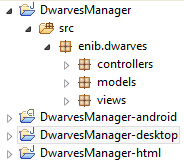
\includegraphics[width=4cm]{img/divers/architecture}
    \caption{Architecture du projet}
		\label{Architecture}
\end{figure}

Le projet est constitué de 4 projets Eclipse, c'est une structure recommandée, lorsque l'on utilise LibGDX en 	vue  d'une application multi-plateforme. Voir figure ~\ref{Architecture}

\begin{description}
\item[DwarvesManager :]C'est le projet principal, qui contient tout le code de l'application, et inclus la librairie GDX.
\item[DwarvesManager-android :]C'est le projet Android, qui référence le projet principal. Il définit toutes les informations pour l’exécution de Dwarves Manager sur le système Android (Manifeste Android), contient également les sources compilées utilisées par LibGdx pour s’exécuter sur Android, ainsi que les librairies du SDK Android. Un seul fichier de code est présent, c'est une classe qui étend la classe AndroidApplication du SDK, afin de pouvoir lancer le jeu.
\item[DwarvesManager-desktop :] Le principe est le même sauf que ce projet contient un main capable d'exécuter l'application sous Windows, Linux et MacOs.
\item[DwarvesManager-html :]Même principe encore, on a ici une classe qui étend GwtApplication du framework Gwt (Google Web Toolkit), qui permet d'inclure le jeu dans une page web et de le faire exécuter par un navigateur internet.
\end{description}

NB : LibGDX nous avait également généré un projet IOs (Pour Iphone/Ipad), mais n'ayant pas le budget pour acheter une licence de développement, nous avons préférer abandonner la compatibilité avec cette plate-forme.

\section*{MVC :}

Nous avons choisi le pattern MVC comme modèle d'architecture, car c'est une solution relativement simple qui nous permet néanmoins d'assurer une bonne extensibilité de notre programme.

\newpage

\chapter*{Modélisation}
\addcontentsline{toc}{chapter}{Modélisation}

\section*{Diagrammes de classe}
\addcontentsline{toc}{section}{Diagrammes de classe}

Sur les diagrammes nous ne montrons pas les liens entre les \og modèles \fg et leurs \og vues \fg. Nous ne détaillerons pas ici les vues. Les attributs montrés publics seront implémenté comme étant privé ou protégé dans le code selon les cas, mais disposerons d'accesseurs et modifieurs publics. Les modifieurs et accesseurs ne sont par conséquent pas non plus détaillés.

Il nous était impossible de représenter toute l'architecture sur un seul diagramme de classe, nous avons donc essayer de découper au mieux les différentes parties du projet.

\begin{figure}
    \center
    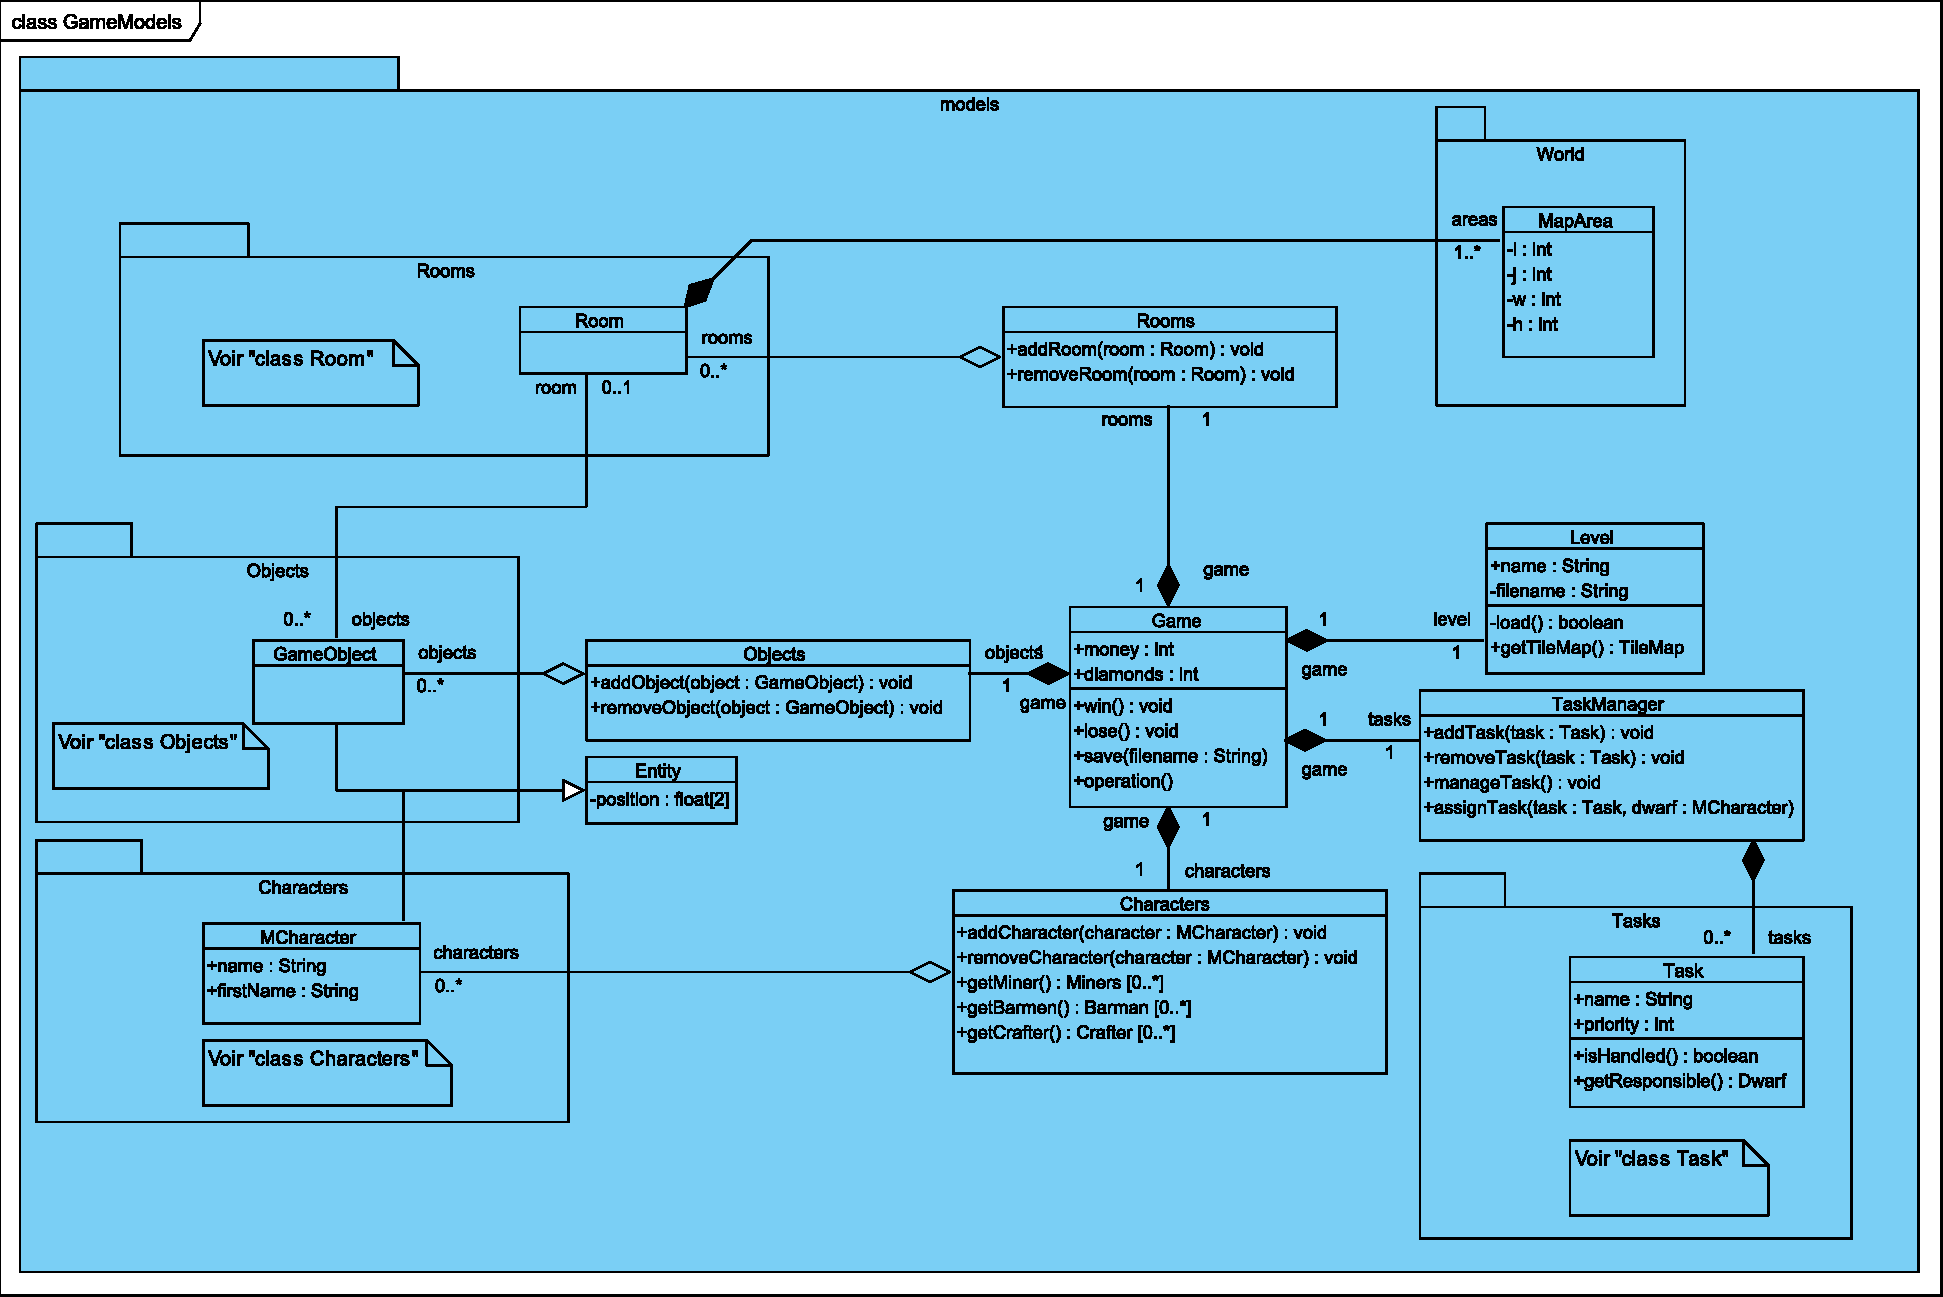
\includegraphics[scale=0.5]{img/class/GameModels}
    \caption{Architecure globale du code métier}
		\label{GameModels}
\end{figure}

\subsection*{class GameModels\\}

Ce diagramme (Figure ~\ref{GameModels}) présente la structure générale de notre code métier.La classe Game est la classe centrale, on l'instancie quand on souhaite créer une nouvelle simulation, elle est composé de plusieurs objets.
\begin{description}
\item [Un \og Characters \fg :] un objet chargé de gérer la population de la simulation
\item [Un \og Rooms \fg :] un objet qui gère toutes les pièces créées par le joueur.
\item [Un \og Objects \fg :] un objet qui gère tout les objets placés par le joueur.
\item [Un \og Level \fg :] un objet qui représente le monde du jeu
\item [Un \og TaskManager \fg :] un objet qui gérera les ordres donnés par le joueur et les attribuera aux nains.
\end{description}

\begin{figure}
    \center
    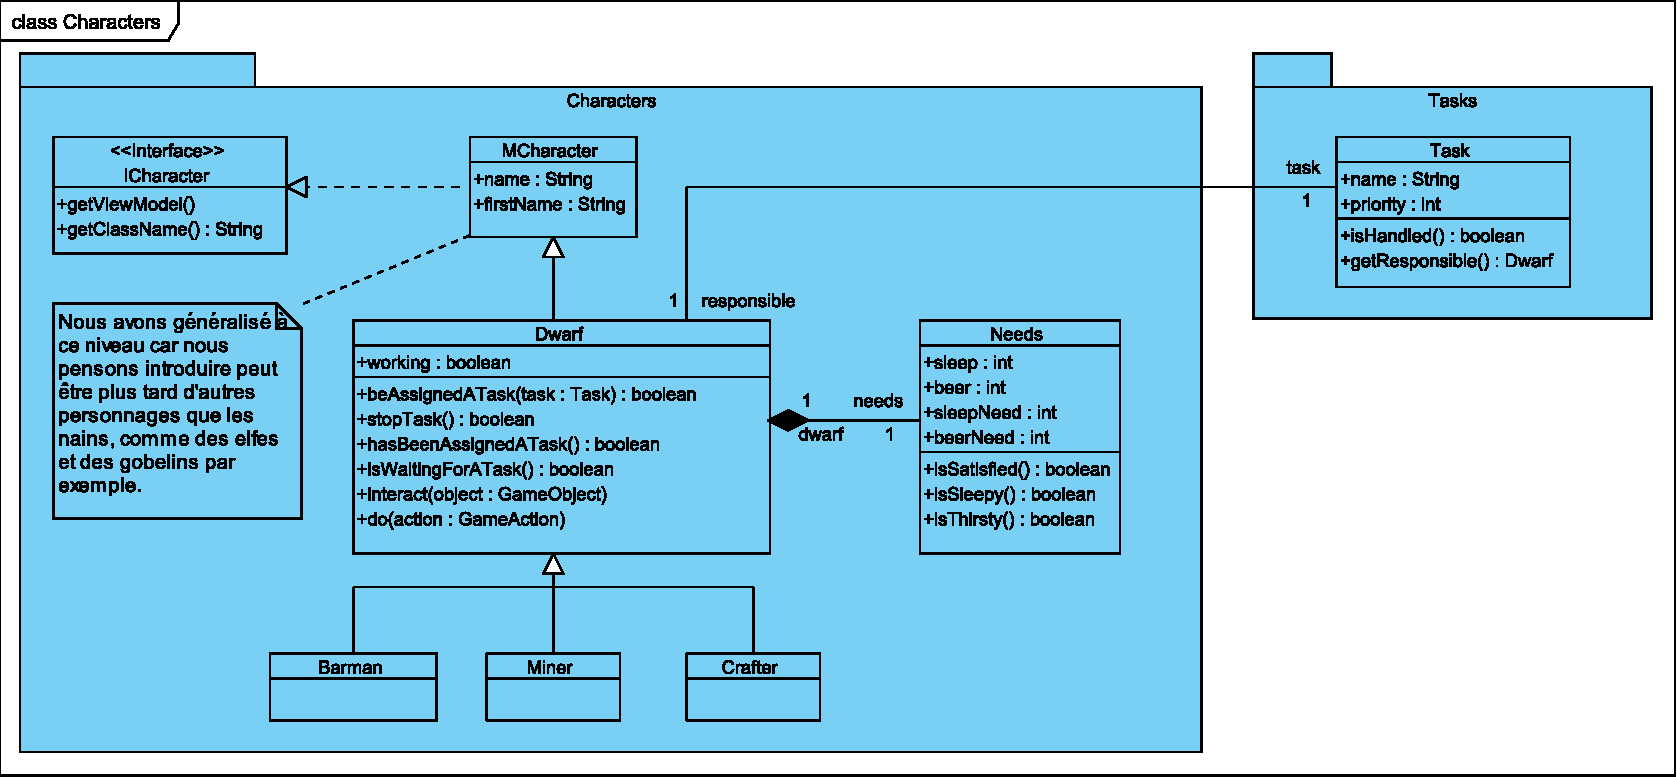
\includegraphics[scale=0.5]{img/class/Characters}
    \caption{Modèle des personnages}
		\label{Characters}
\end{figure}

\begin{figure}
    \center
    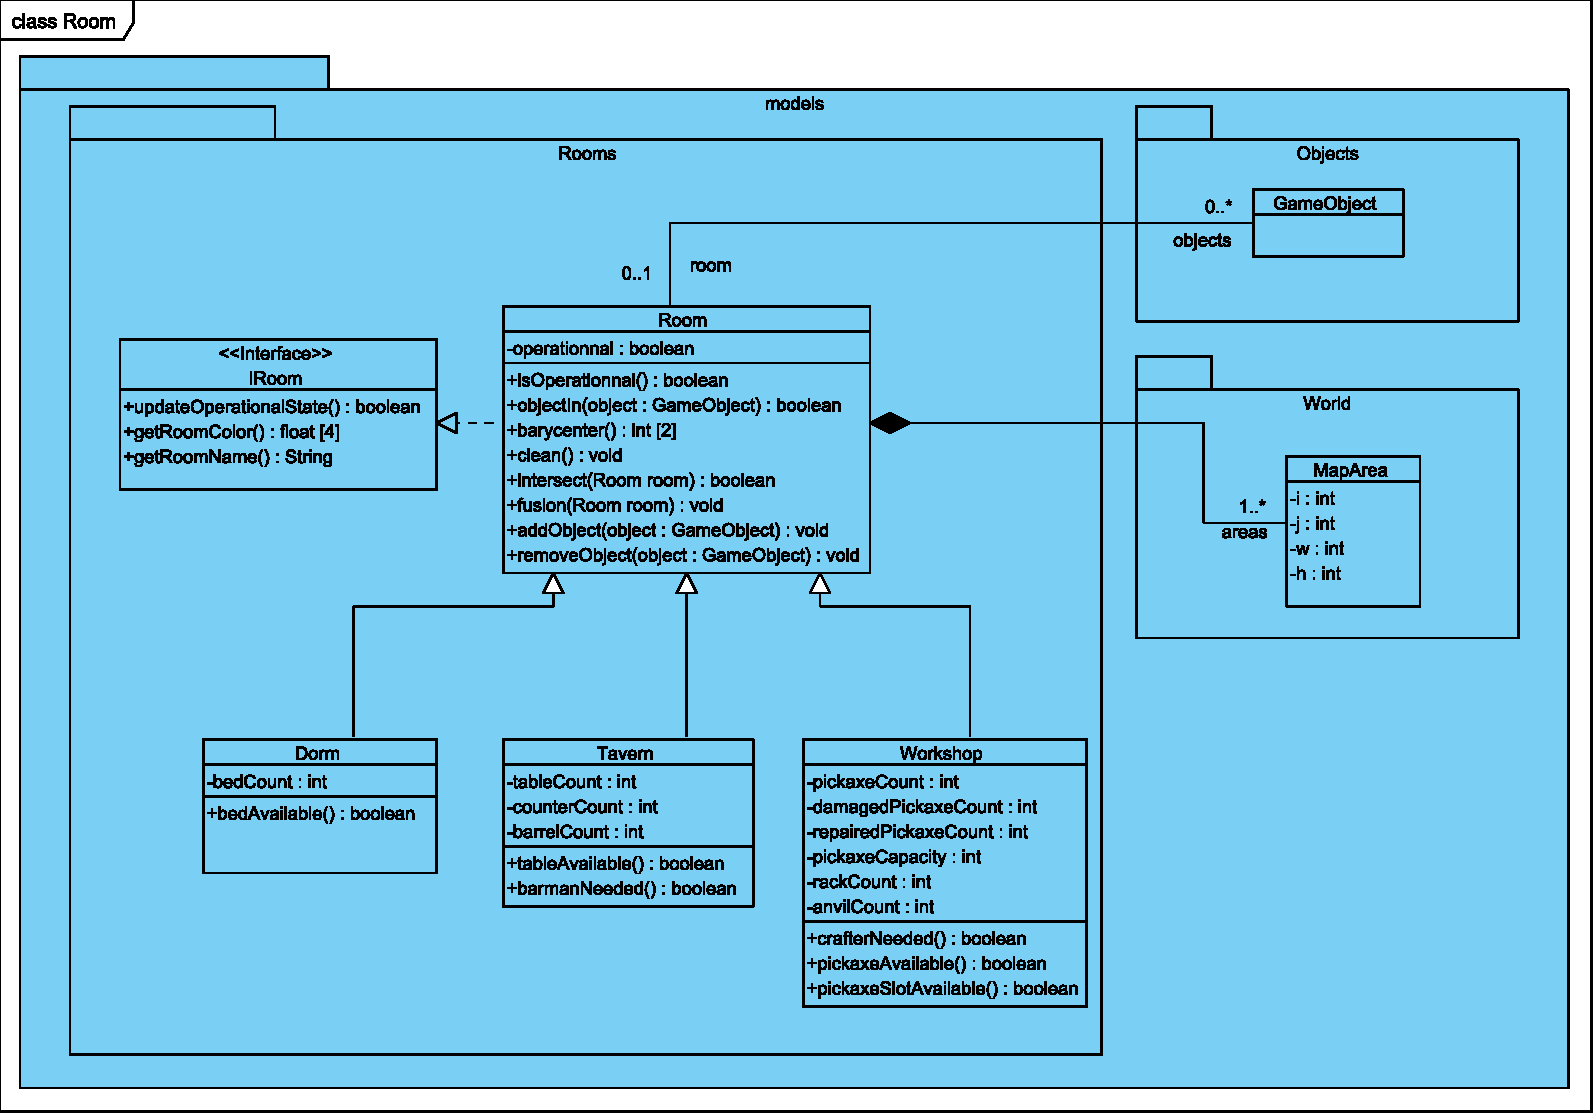
\includegraphics[scale=0.5]{img/class/Room}
    \caption{Modèle des pièces}
		\label{Rooms}
\end{figure}

\begin{figure}
    \center
    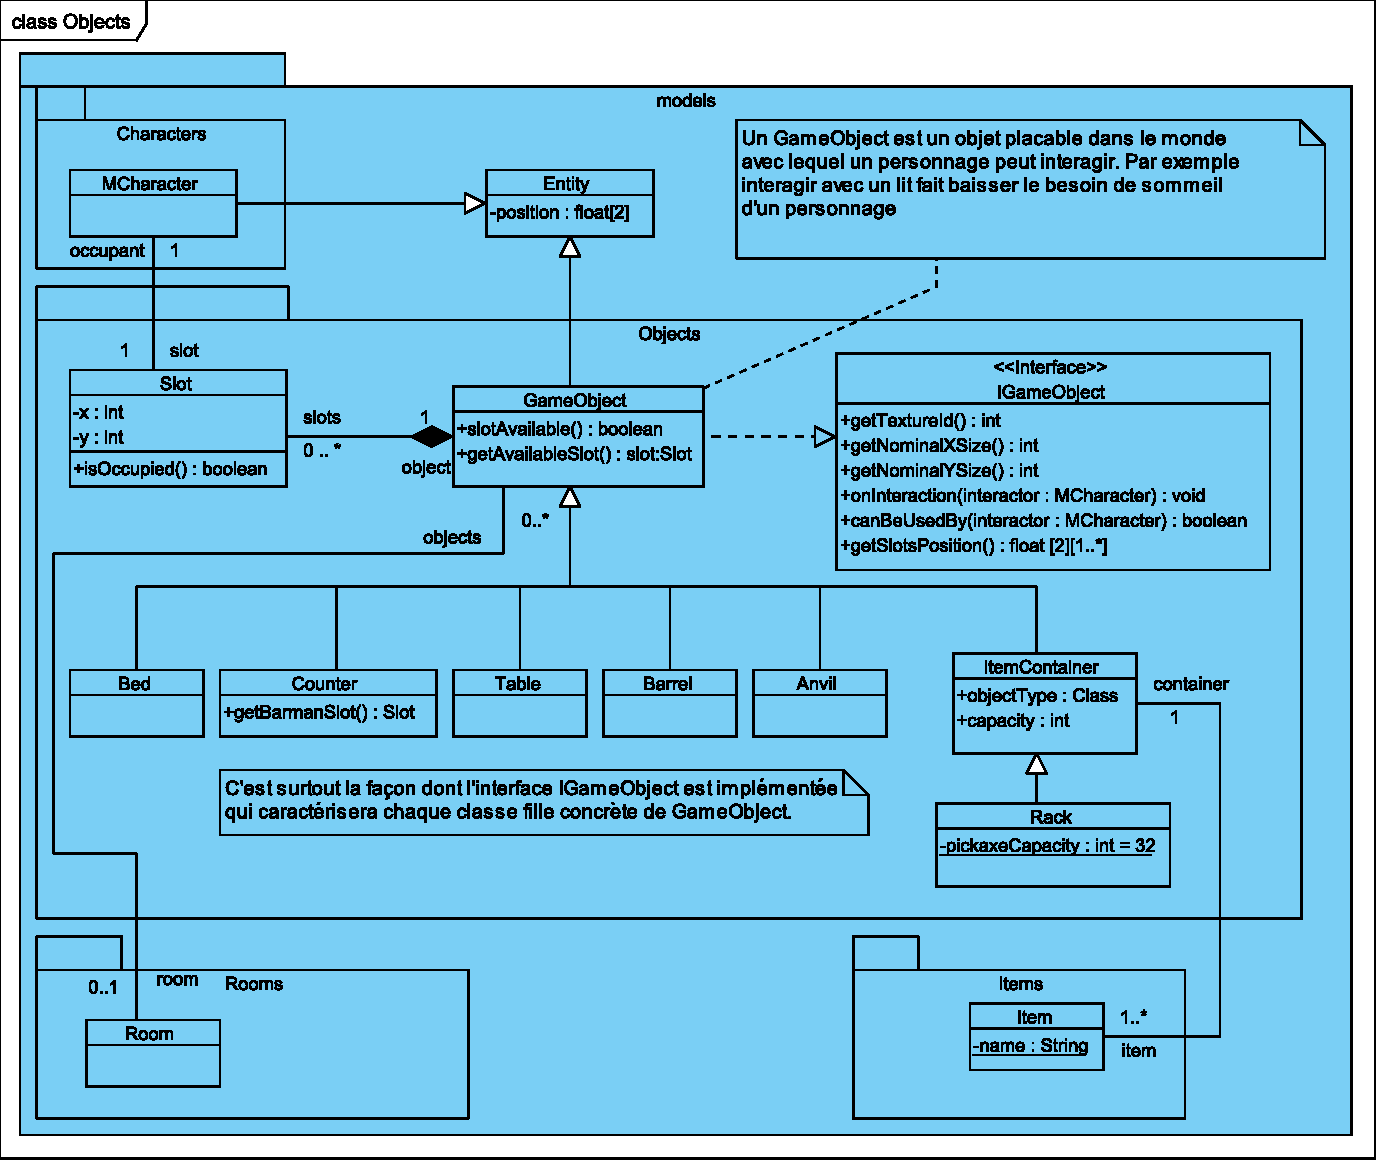
\includegraphics[scale=0.5]{img/class/Objects}
    \caption{Modèle des objets}
		\label{GameObjects}
\end{figure}

\begin{figure}
    \center
    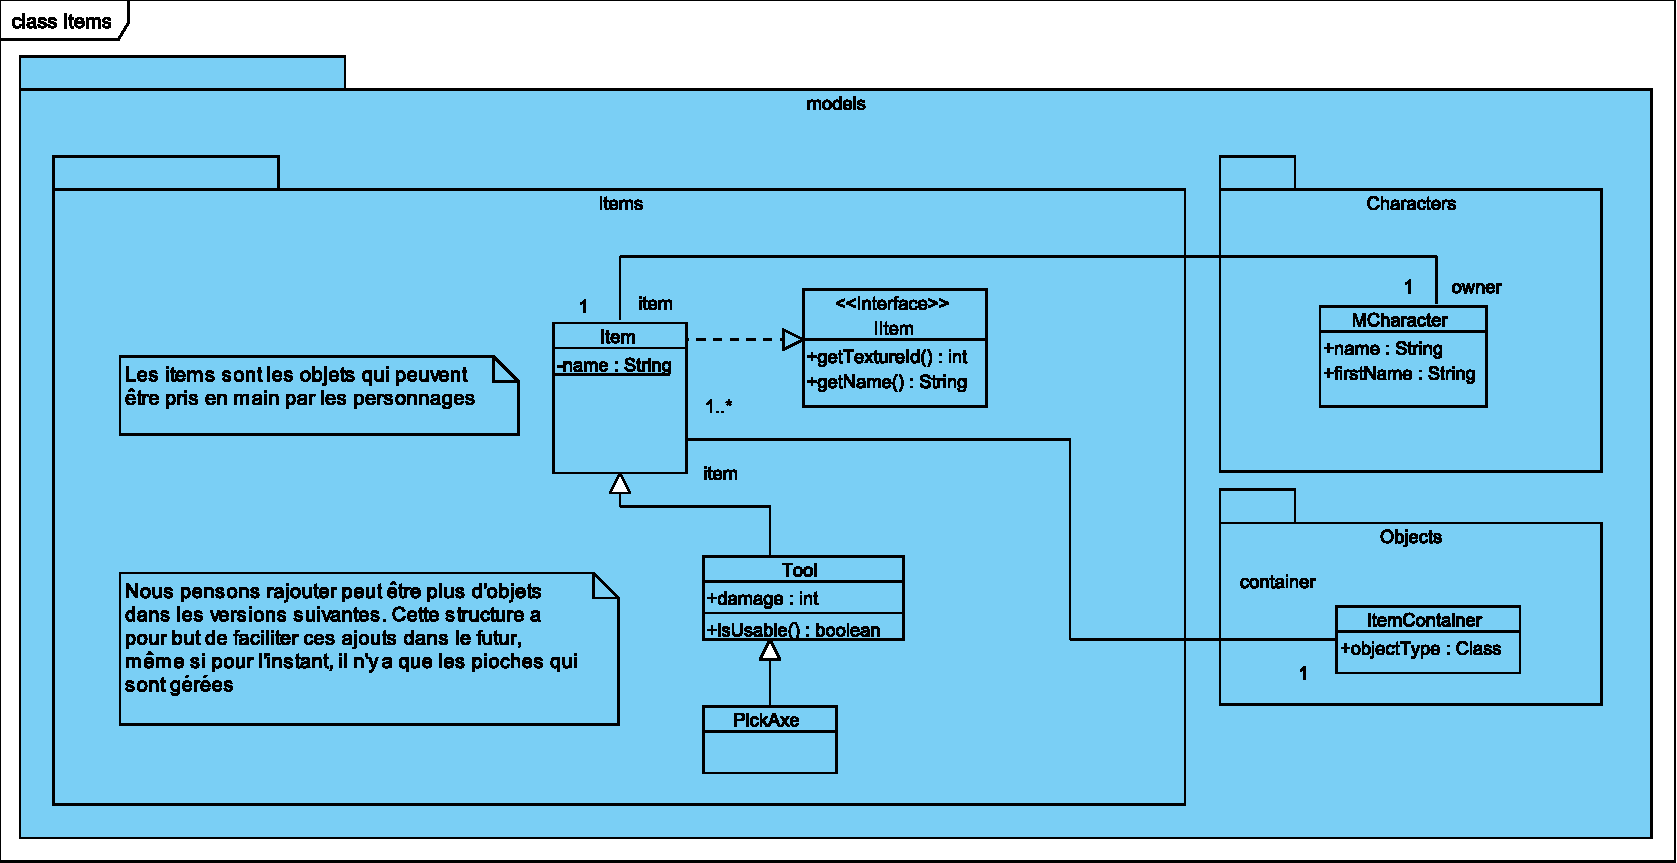
\includegraphics[scale=0.5]{img/class/Items}
    \caption{Modèle des items}
		\label{Items}
\end{figure}

\begin{figure}
    \center
    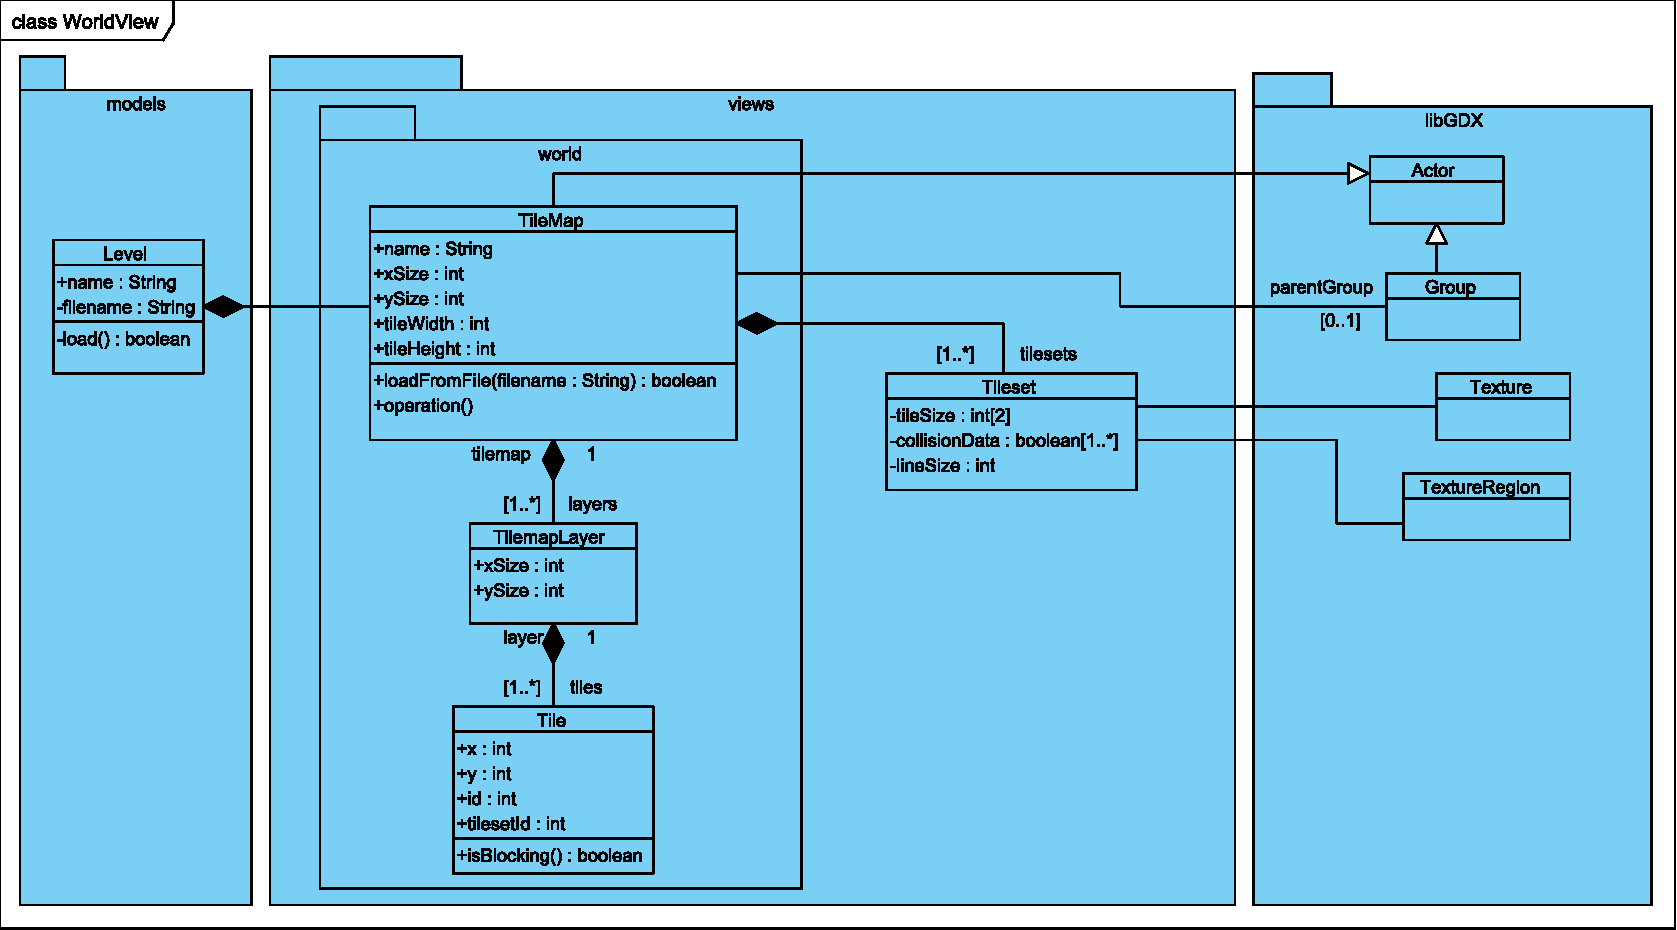
\includegraphics[scale=0.5]{img/class/WorldView}
    \caption{Modèle d'affichage du monde}
		\label{WorldView}
\end{figure}

\begin{figure}
    \center
    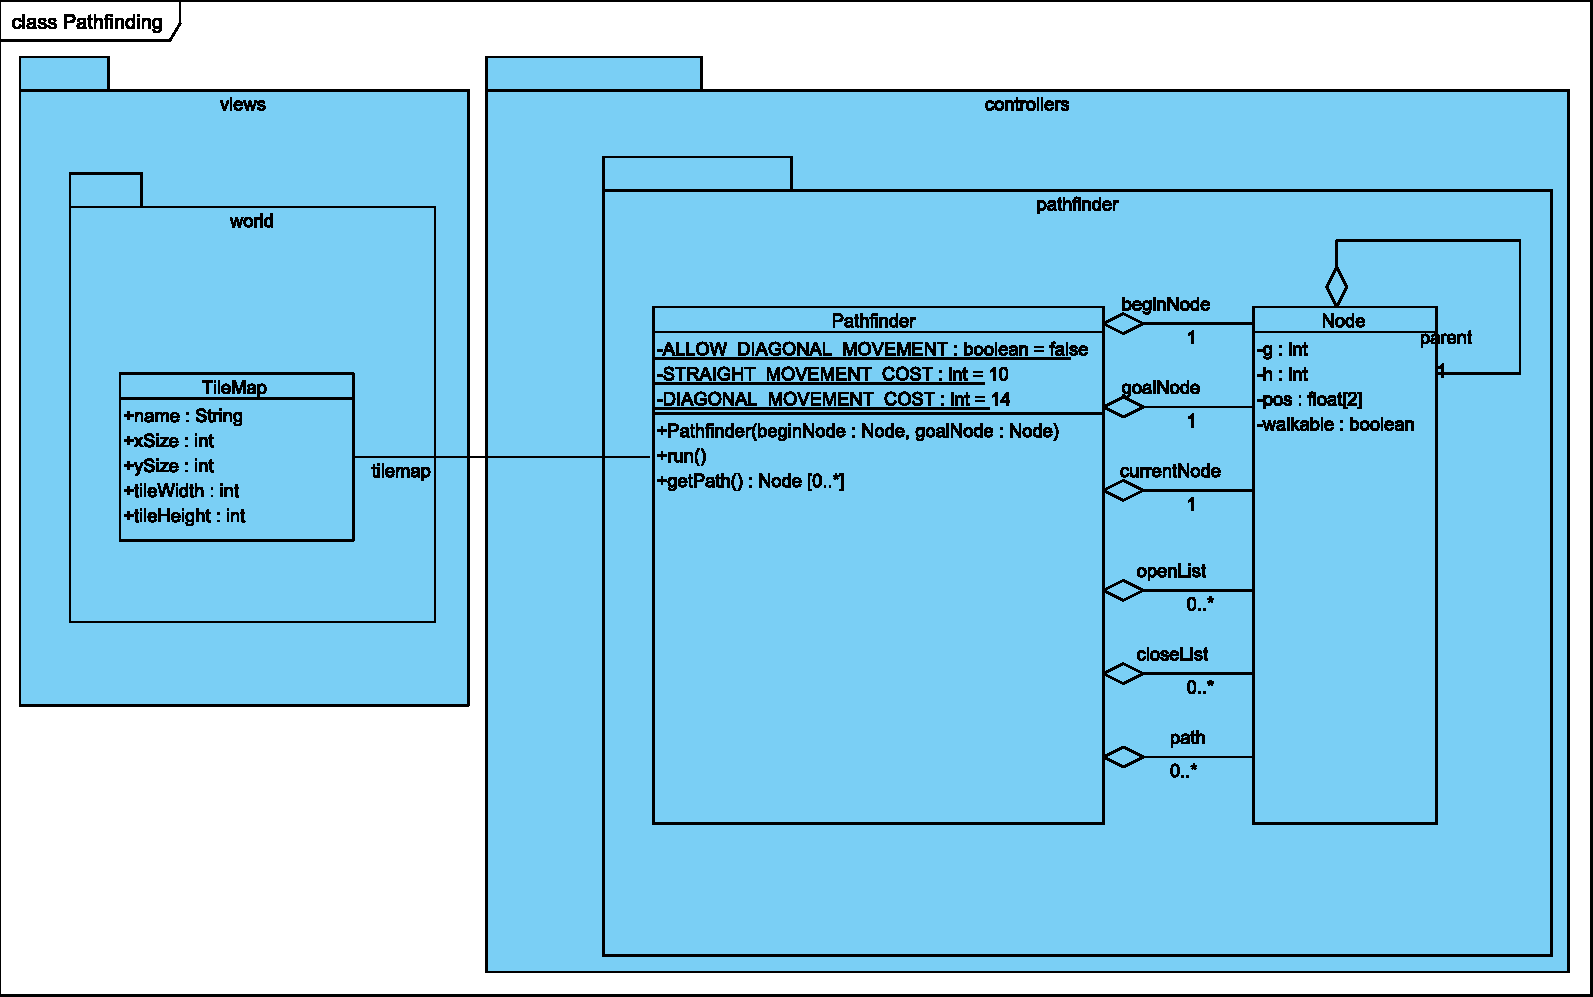
\includegraphics[scale=0.5]{img/class/Pathfinding}
    \caption{Modèle du pathfinder}
		\label{Pathfinding}
\end{figure}

\begin{figure}
    \center
    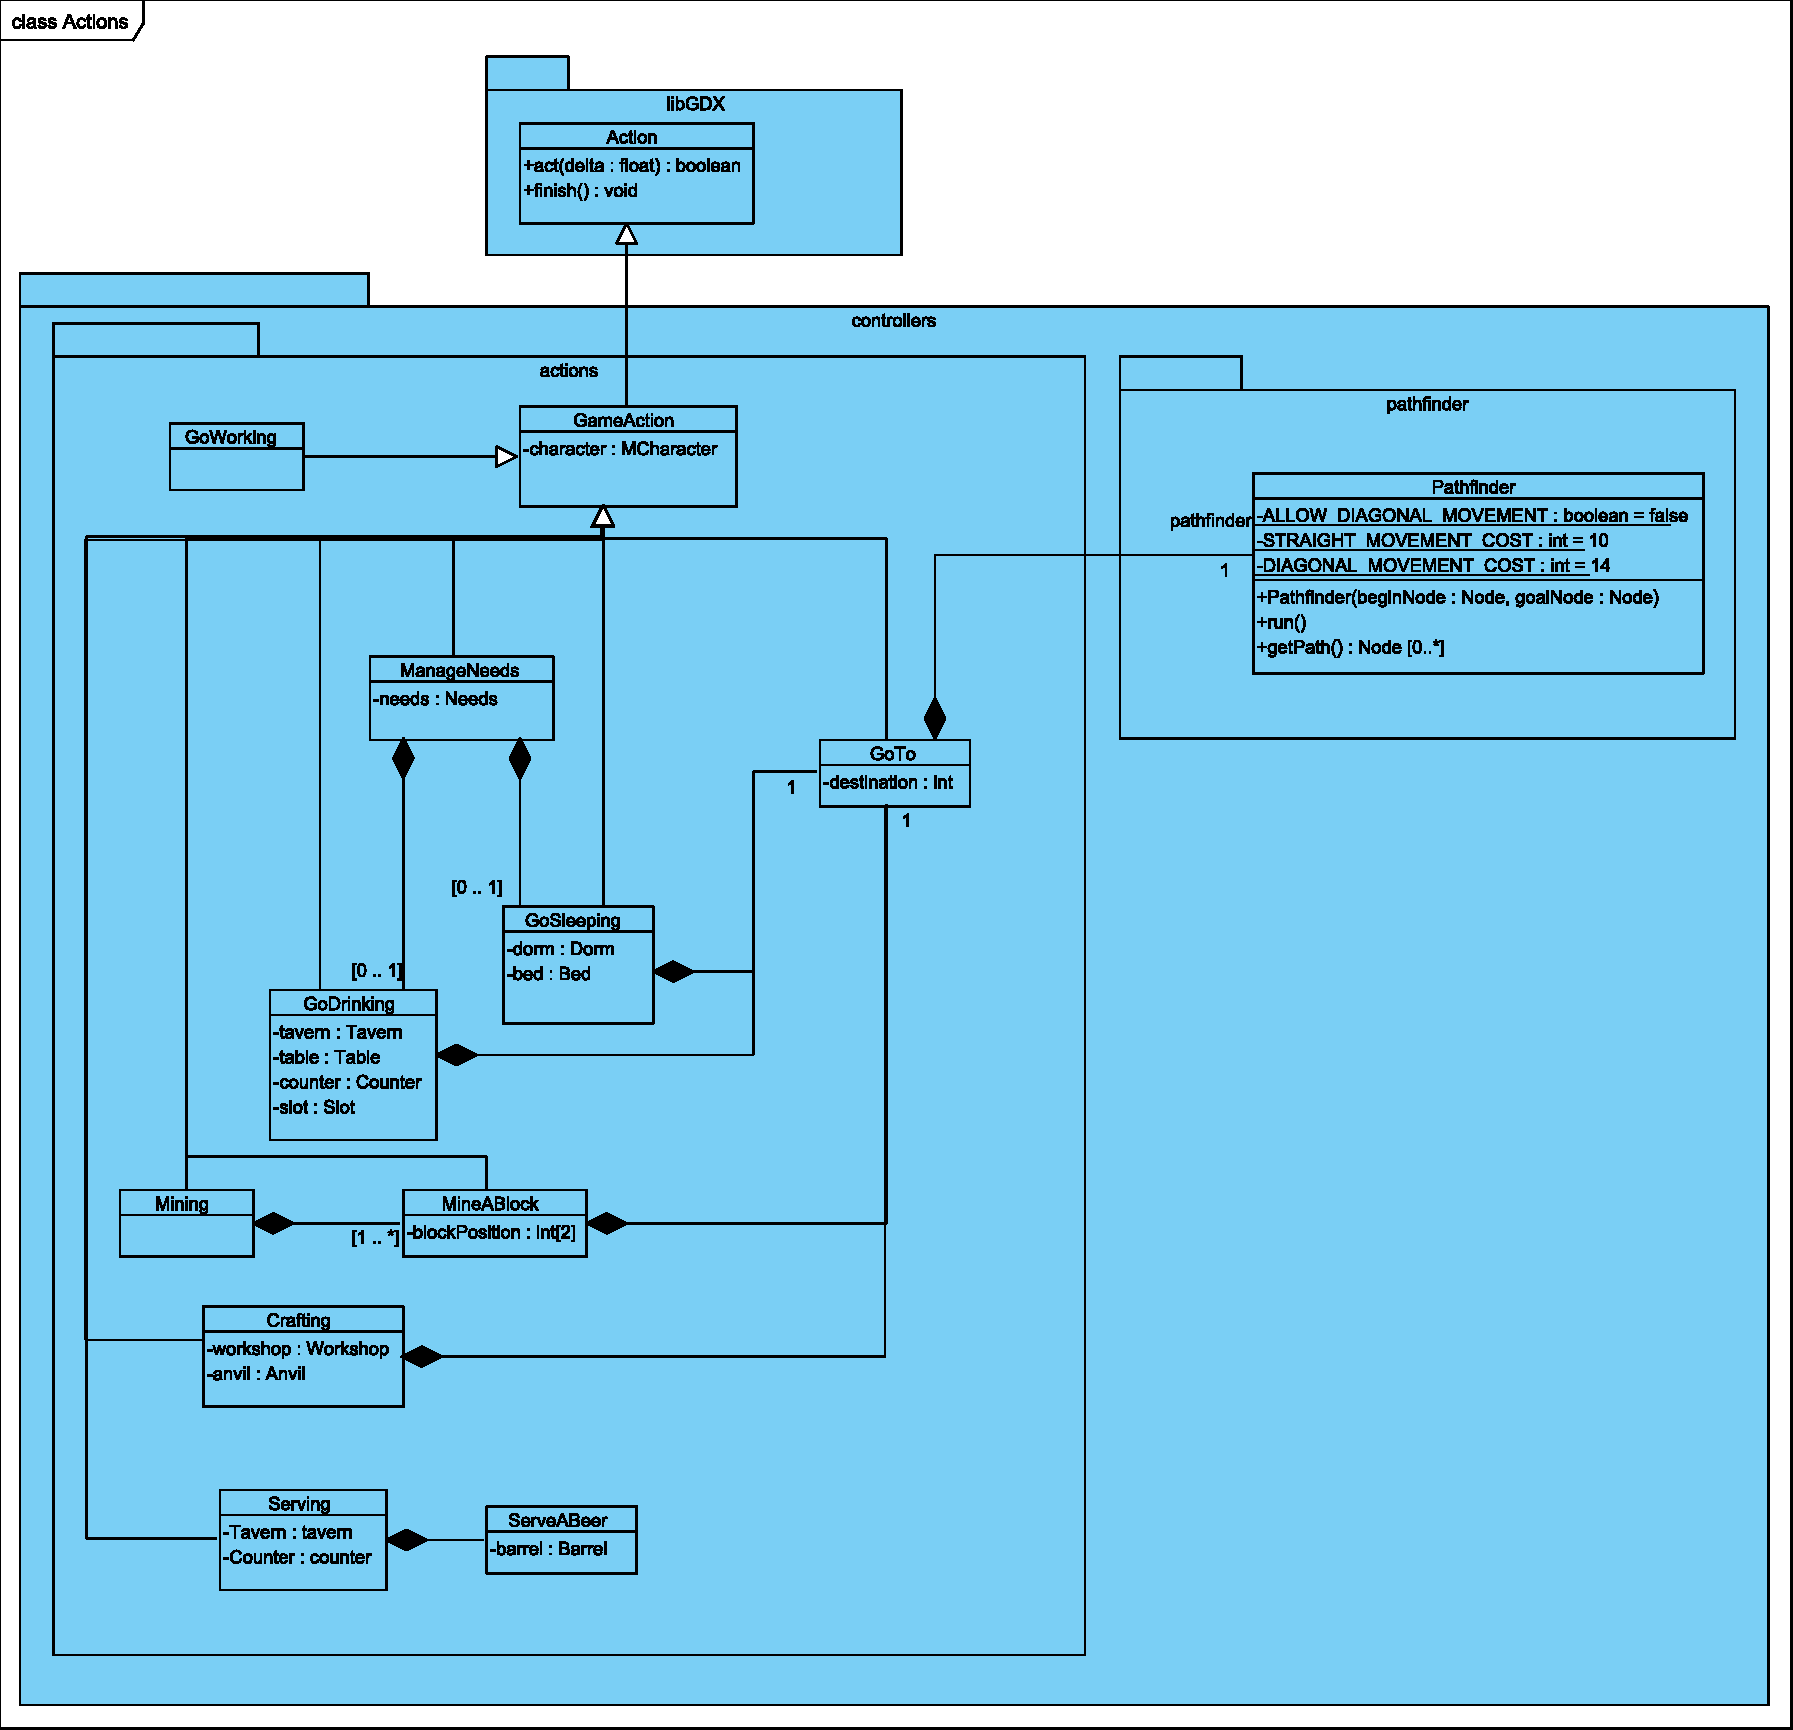
\includegraphics[scale=0.5]{img/class/Actions}
    \caption{Modèle des actions}
		\label{Actions}
\end{figure}

\subsection*{Remarque sur class WorldView (Figure \ref{WorldView})\\}

Comme on peut le voir une partie des données qui constituent le monde sont stockées dans des classes du package view. Ces classes d'affichage avaient déjà été créées par l'un d'entre nous avant le projet, et comme elle fonctionnaient bien, nous avons choisis de les réutiliser. Néanmoins, elles n'ont pas été conçues pour une architecture MVC, le but de la classe Level est donc de servir d'interface entre les modèles et les données contenues dans ces classes.

\subsection*{Remarque sur class Pathfinding (Figure \ref{Pathfinding})\\}

Le pathfinder utilise l'algorithme A*, d'où cette structure.

\clearpage

\subsection*{Remarque sur class Actions (Figure \ref{Actions})\\}

Ce modèle a été conçu en ayant en tête la façon dont fonctionne les \og Actions \fg de LibGdx. Dans LibGdx, il nous suffira grossièrement de faire :

\vspace{0.5cm}

\begin{lstlisting}
model.getView().addAction(new Action(model));
\end{lstlisting}

\vspace{0.5cm}

Cela aura pour effet d'ajouter une action à réaliser au modèle et à sa vue.
Ces actions peuvent être parallélisées ou organisées en séquence de manière très simple grâce à libGdx.

Par exemple dans le code de l'action ManageNeeds on aura :

\vspace{0.5cm}

\begin{lstlisting}
public void entry(){
	this.target.clearActions() // Le nain stoppe tout pour passer a la gestion de ses besoins
	this.goSleep = new GoSleeping(this.target);
	this.goDrink = new GoDrinking(this.target);
	this.target.getView().addAction(this.goSleep)
	this.target.getView().addAction(this.goDrink) // Ce n'est pas le code final, mais un exemple bien sur
}
\end{lstlisting}


\vspace{0.5cm}

De ce principe découle tout le système de composition mis en place dans ce diagramme.\\

\vspace{0.4cm}

\bsc{NB :} Nous pensons que donner une idée de ce à quoi ressemblera le code permet de mieux comprendre ce diagramme.

\clearpage
\section*{Diagrammes d'activités}
\addcontentsline{toc}{section}{Diagrammes d'activités}

\begin{figure}[bh]
    \center
    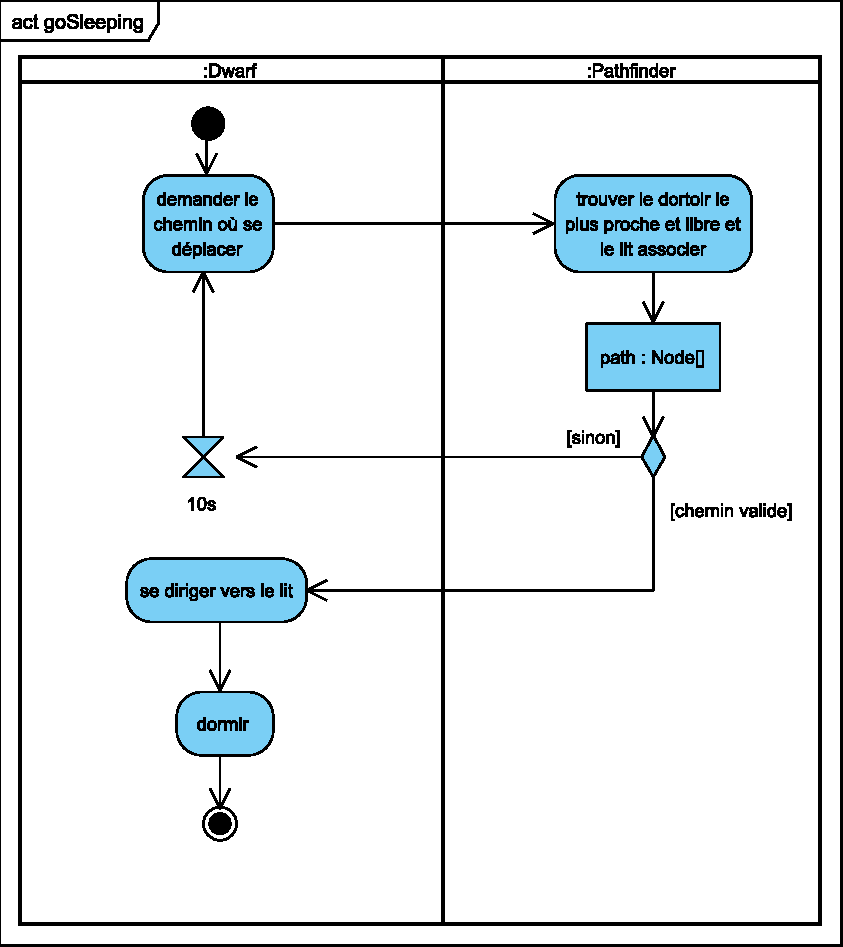
\includegraphics[width=15cm]{img/act/goSleeping}
    \caption{Activité aller dormir}
		\label{}
\end{figure}

\begin{figure}[H]
    \center
    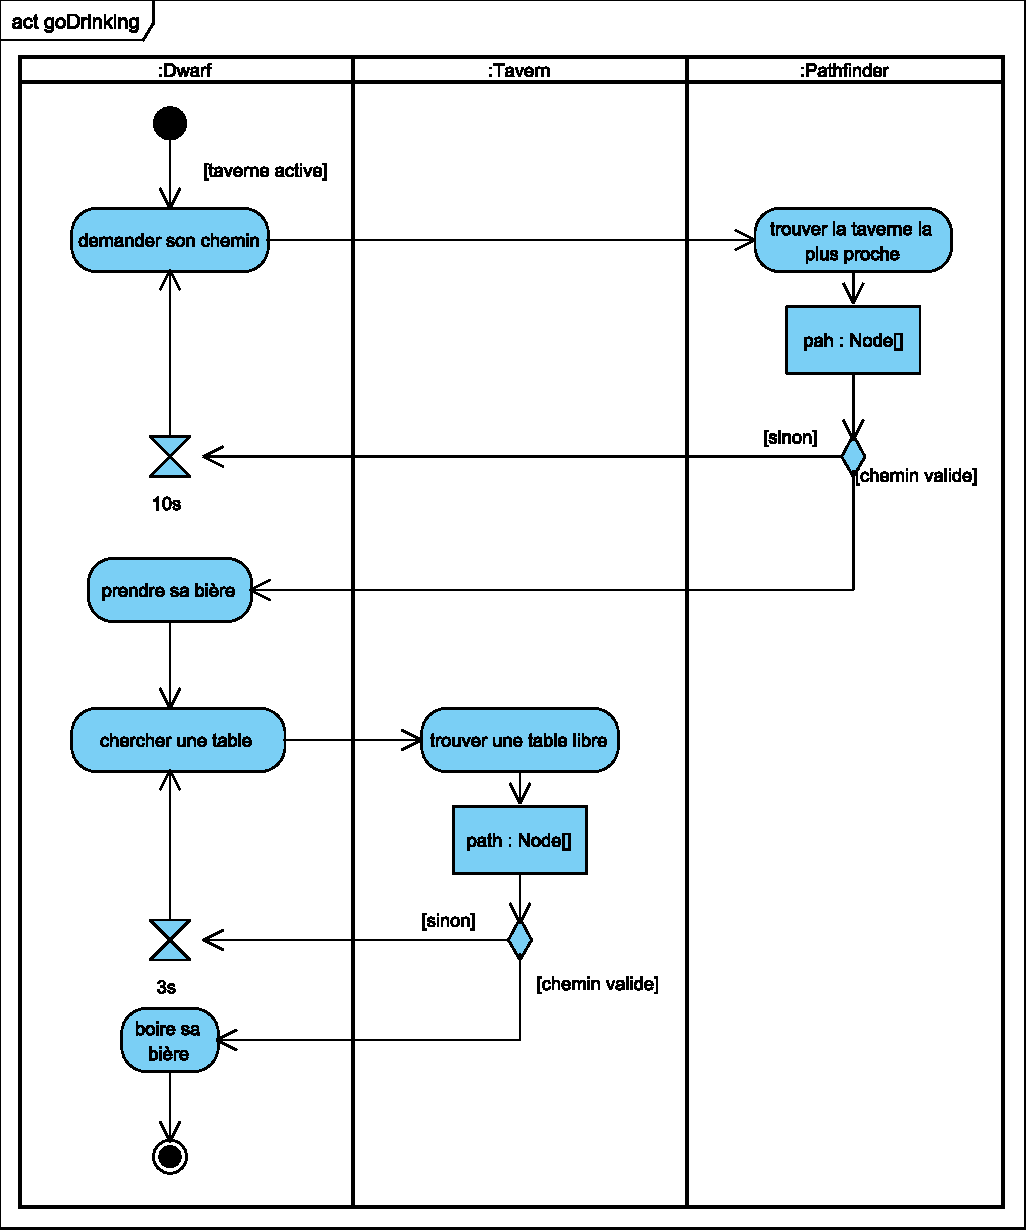
\includegraphics[width=15cm]{img/act/goDrinking}
    \caption{Activité aller boire}
		\label{}
\end{figure}


\begin{figure}[H]
		\center
    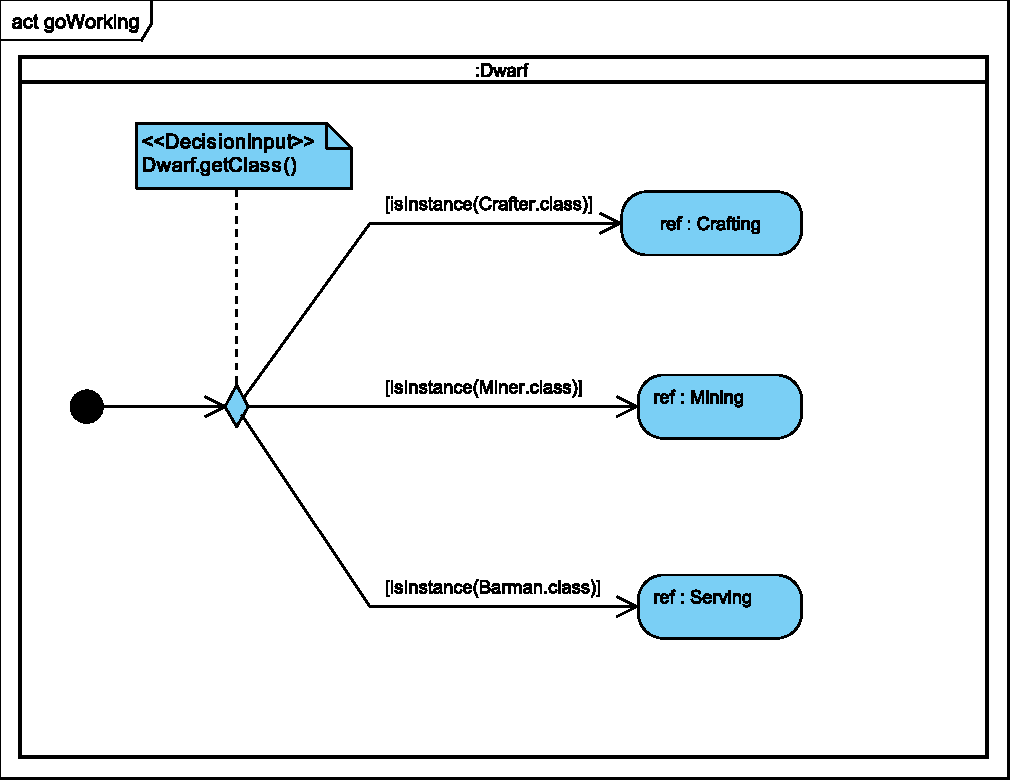
\includegraphics[width=15cm]{img/act/goWorking}
    \caption{Activité aller travailler}
		\label{}
\end{figure}

\begin{figure}[H]
    \center
    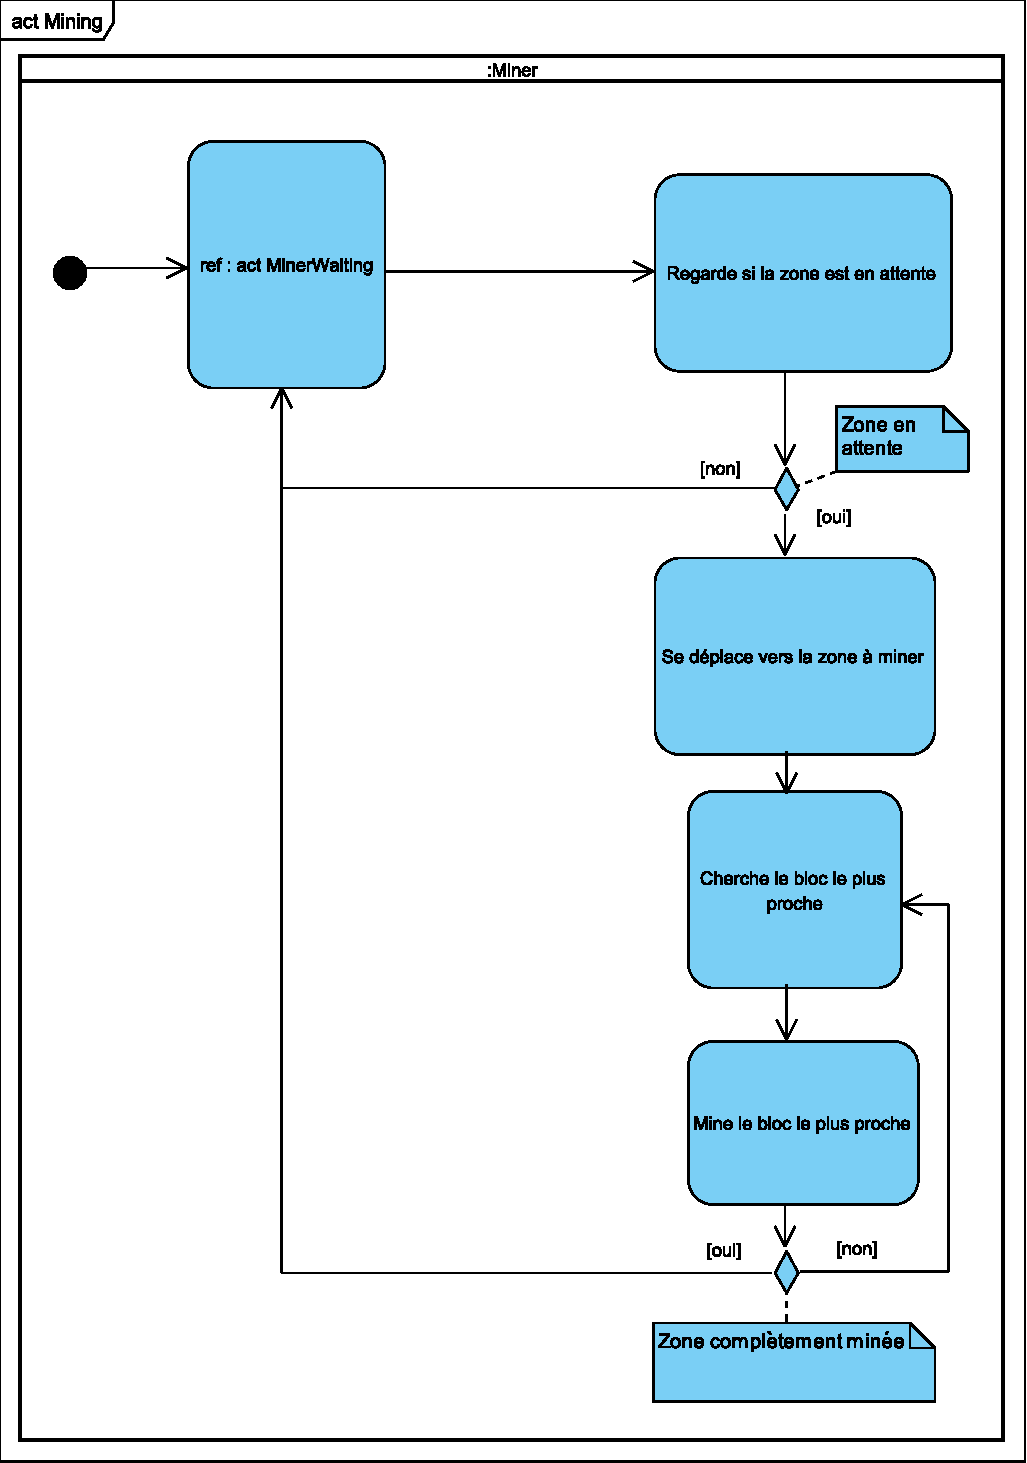
\includegraphics[width=15cm]{img/act/Mining}
    \caption{Activité aller miner}
		\label{}
\end{figure}


\begin{figure}[H]
    \center
    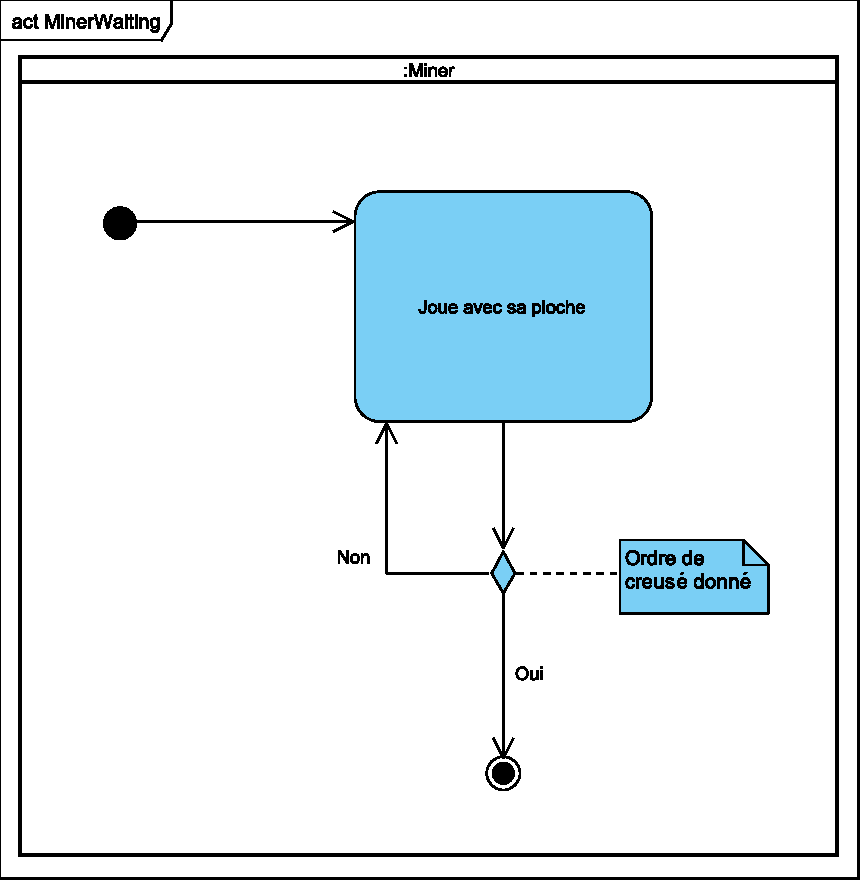
\includegraphics[width=15cm]{img/act/MinerWaiting}
    \caption{Activité d'attente du mineur}
		\label{}
\end{figure}


\begin{figure}[H]
    \center
    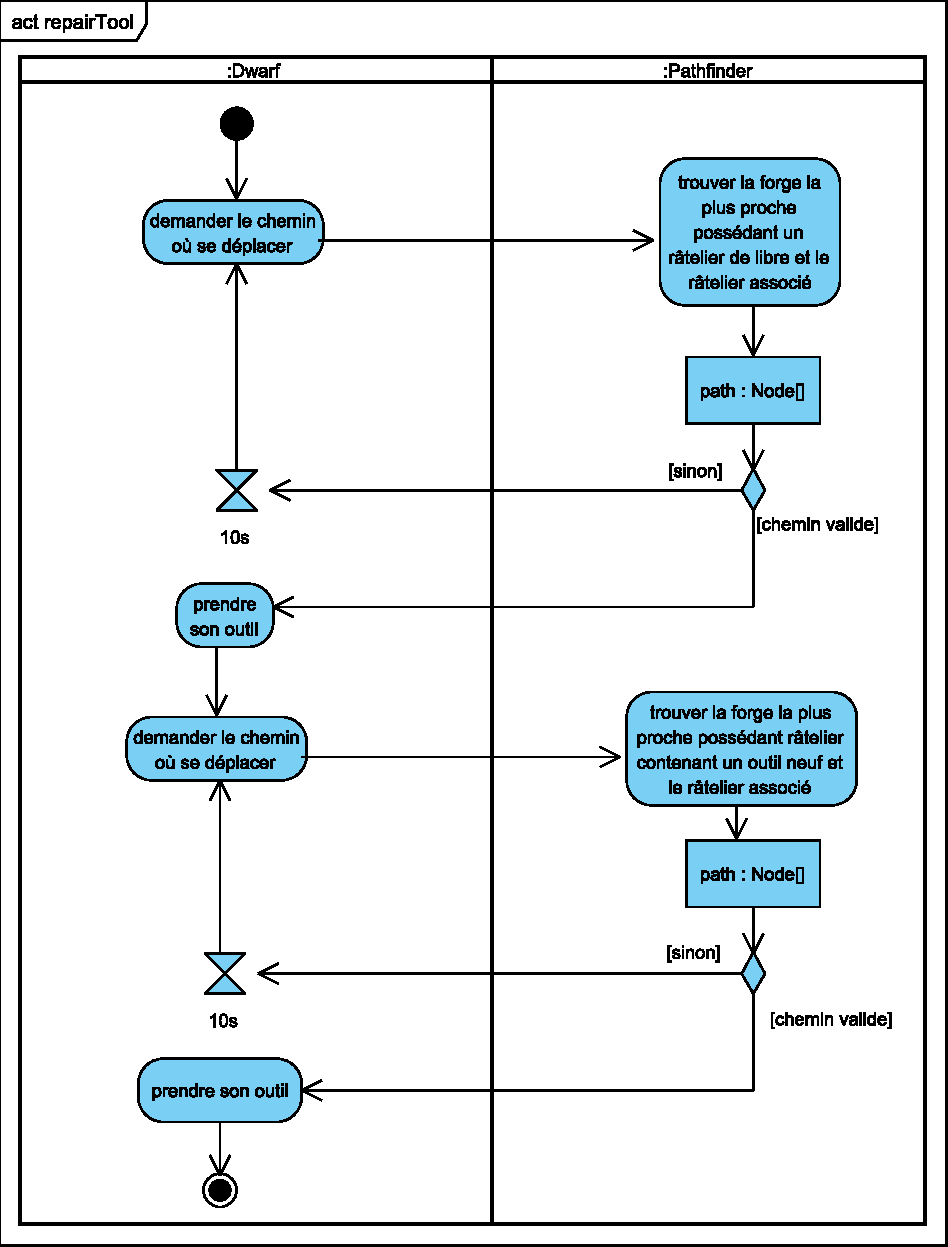
\includegraphics[width=15cm]{img/act/repairTool}
    \caption{Activité aller réparer son outil}
		\label{}
\end{figure}


\begin{figure}[H]
    \center
    \includegraphics[width=15cm]{img/act/workshopNewTool}
    \caption{Activité de recherche de l'atelier le plus proche possédant au moins un outil neuf}
		\label{}
\end{figure}


\begin{figure}[H]
    \center
    \includegraphics[width=15cm]{img/act/workshopFree}
    \caption{Activité de recherche de l'atelier le plus proche possédant au moins un râtelier libre}
		\label{}
\end{figure}


\begin{figure}[H]
    \center
    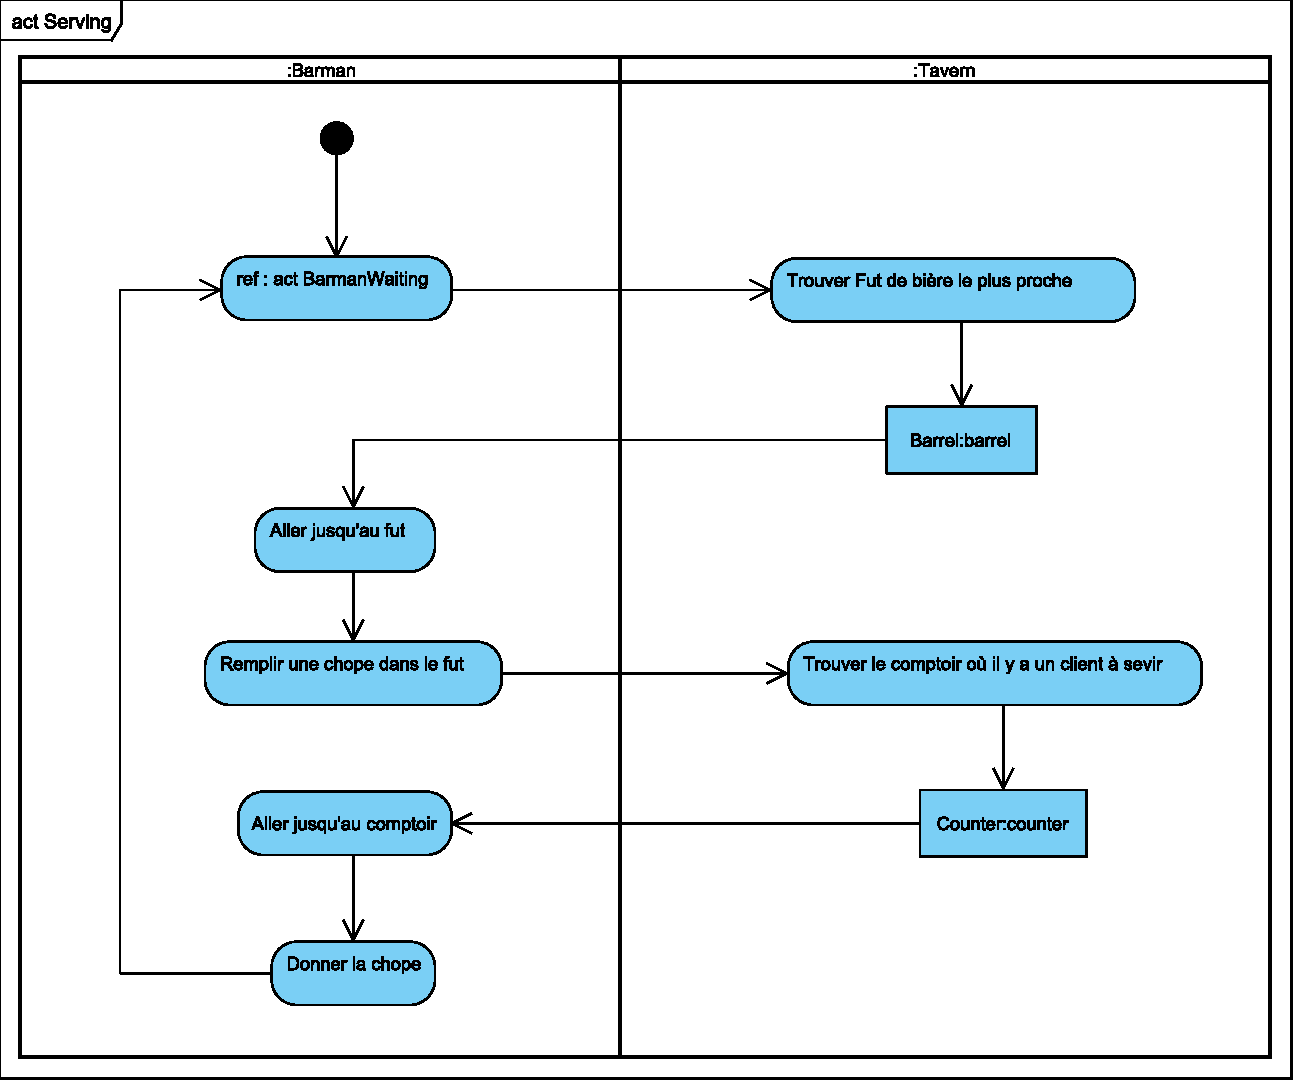
\includegraphics[width=15cm]{img/act/Serving}
    \caption{Activité de travail du barman}
		\label{}
\end{figure}


\begin{figure}[H]
    \center
    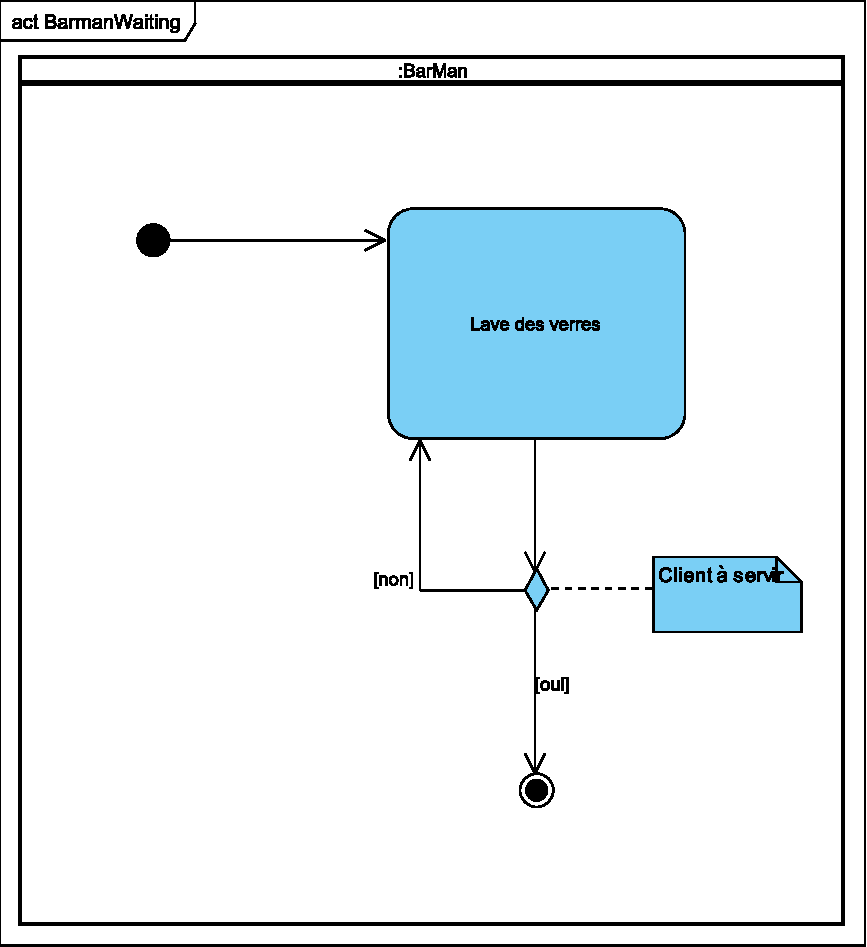
\includegraphics[width=15cm]{img/act/BarmanWaiting}
    \caption{Activité d'attente du barman}
		\label{}
\end{figure}

\begin{figure}[H]
    \center
    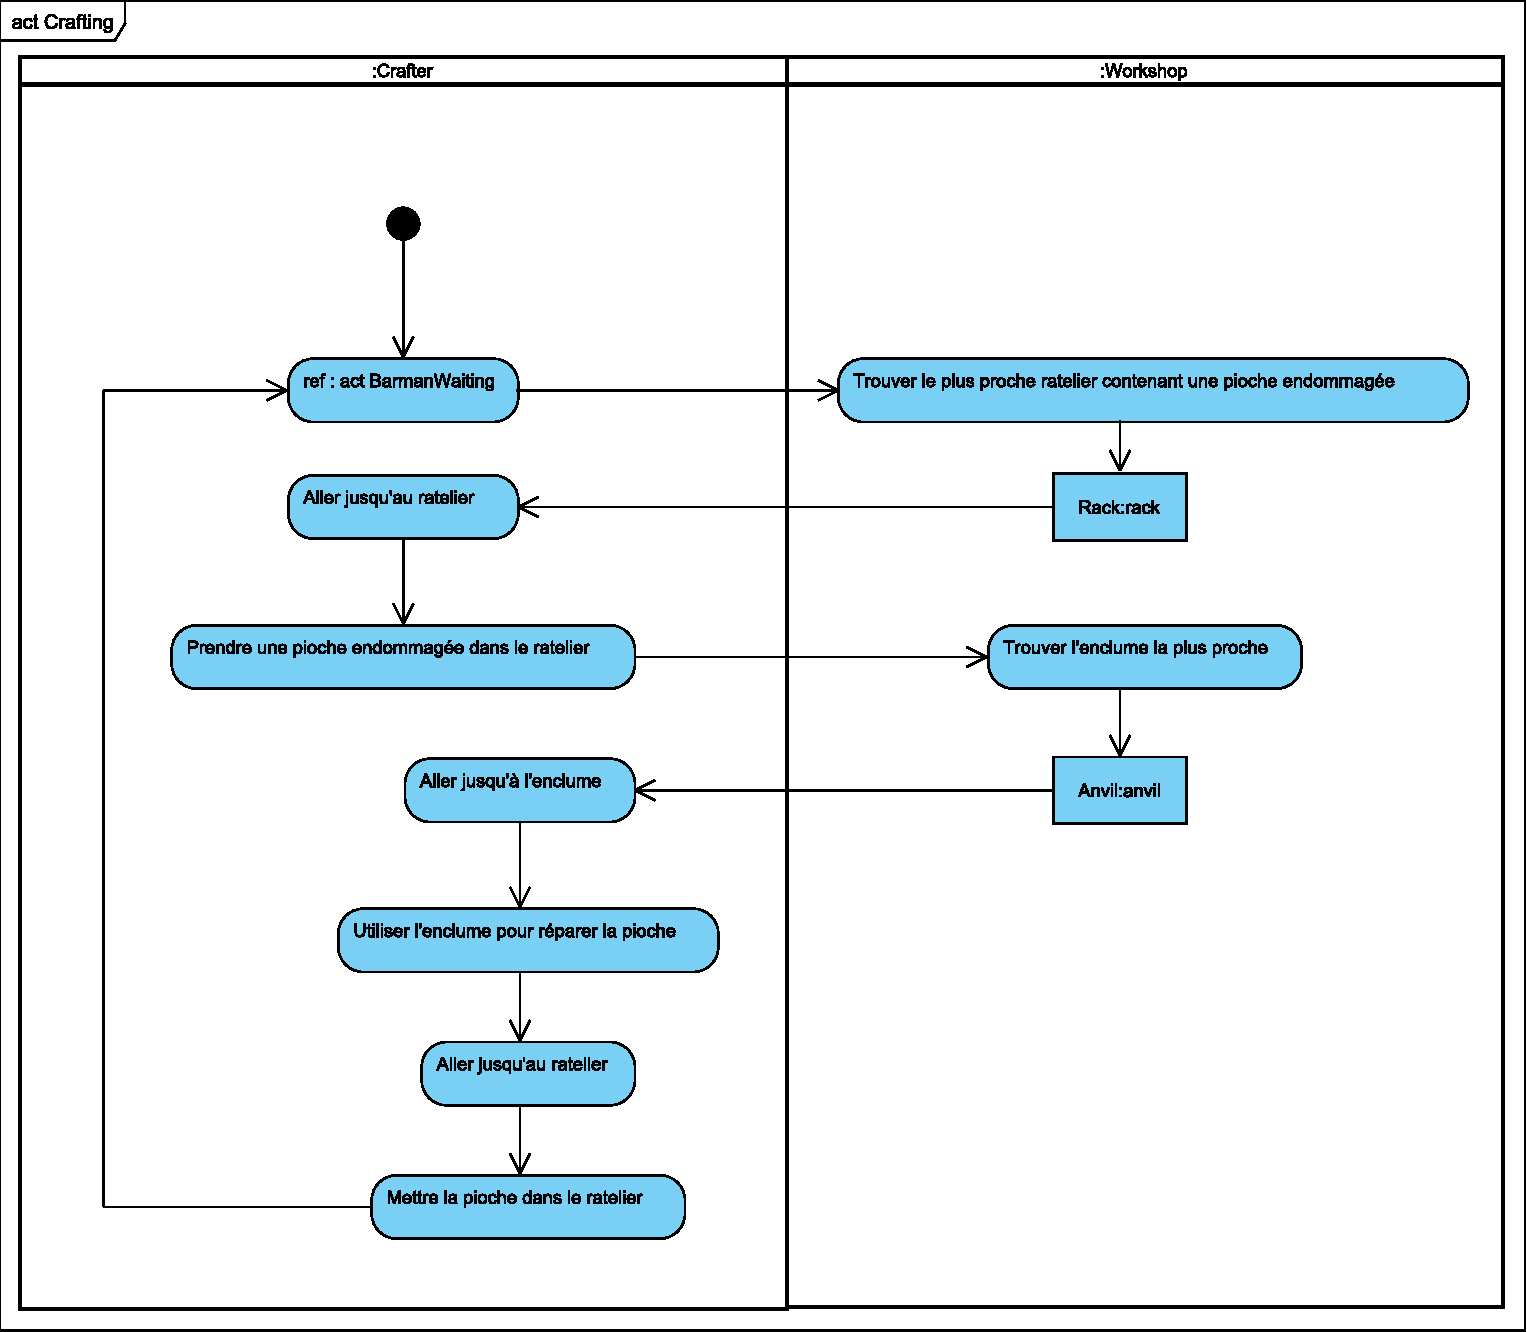
\includegraphics[width=15cm]{img/act/Crafting}
    \caption{Activité de travail de l'artisan}
		\label{}
\end{figure}

\begin{figure}[H]
    \center
    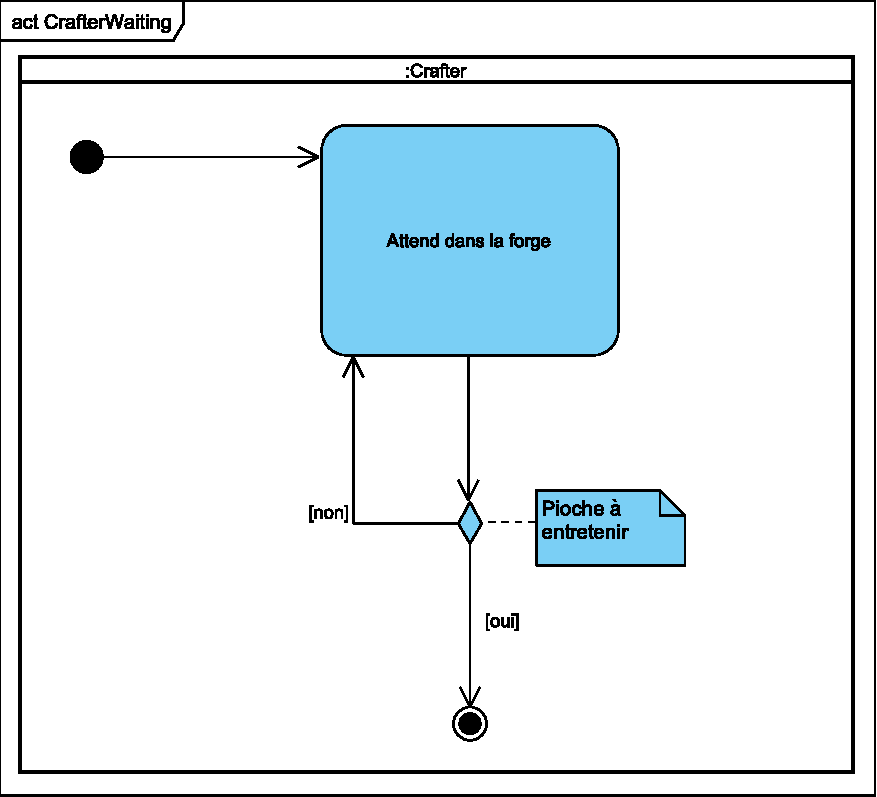
\includegraphics[width=15cm]{img/act/CrafterWaiting}
    \caption{Activité d'attente de l'artisan}
		\label{}
\end{figure}

\clearpage
\section*{Machines à états}
\addcontentsline{toc}{section}{Machine à états}

\begin{figure}[bh!]
    \center
    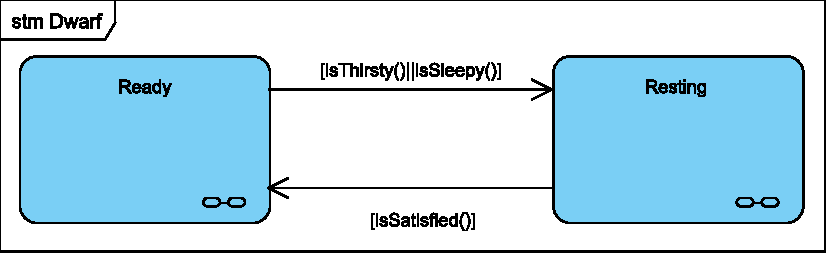
\includegraphics[width=15cm]{img/stm/Dwarf}
    \caption{Machine à états du nains}
		\label{}
\end{figure}


\begin{figure}[bh!]
    \center
    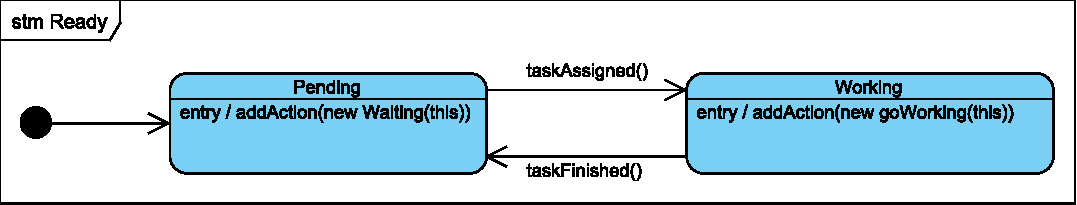
\includegraphics[width=15cm]{img/stm/Ready}
    \caption{Détail de la sous-machine Ready du diagramme Dwarf}
		\label{}
\end{figure}


\begin{figure}[bh!]
    \center
    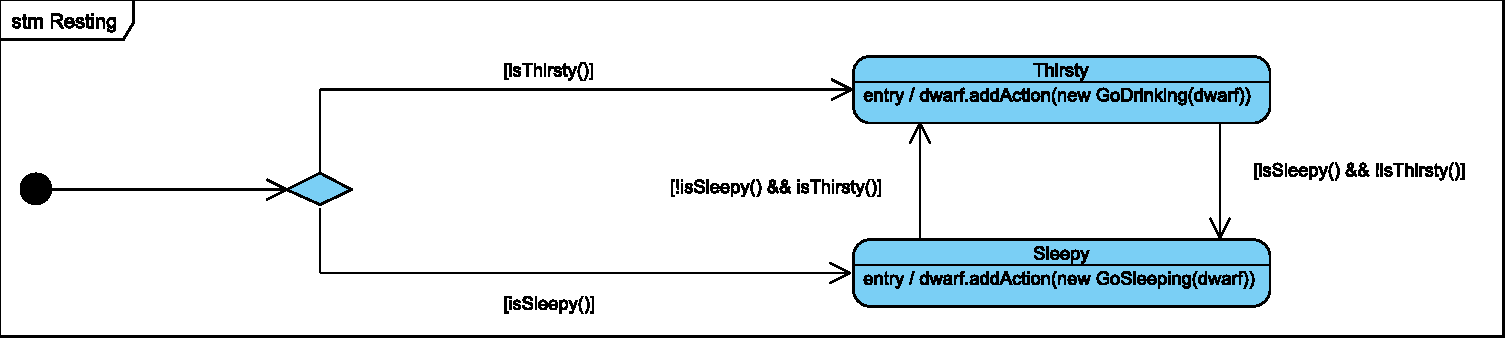
\includegraphics[width=15cm]{img/stm/Resting}
    \caption{Détail de la sous-machine Resting du diagramme Dwarf}
		\label{}
\end{figure}

\begin{figure}[bh!]
    \center
    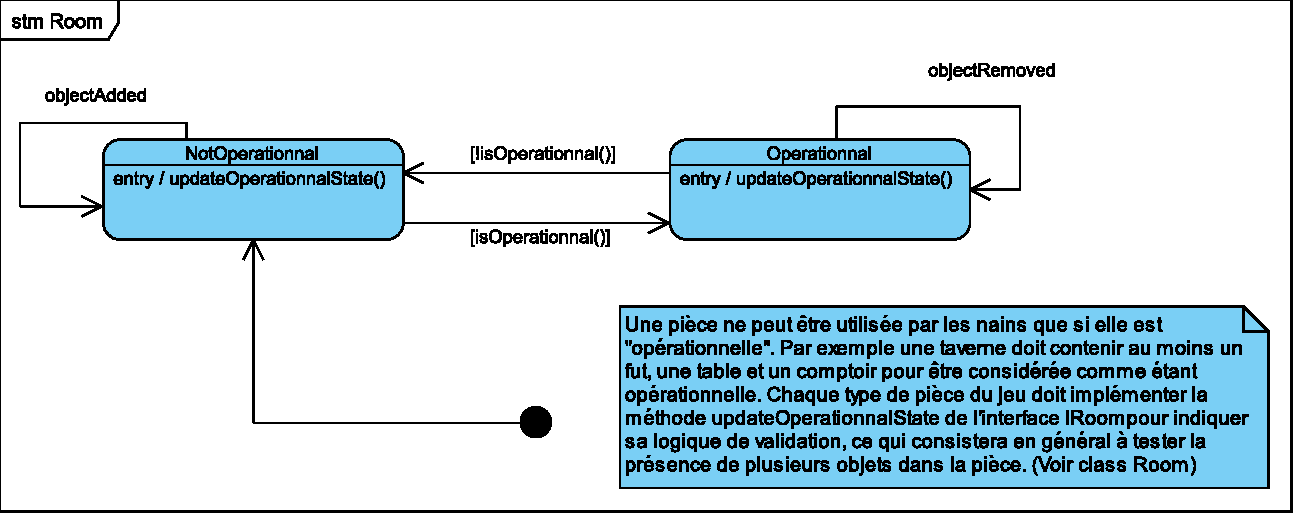
\includegraphics[width=15cm]{img/stm/Room}
    \caption{Machine à état des pièces}
		\label{}
\end{figure}

\clearpage
\begin{figure}[H!]
    \center
    
\includegraphics[scale=2.5]{img/divers/nain}
    \legend{\Huge{Merci d'avoir lu}}
\end{figure}
\end{document}